\documentclass[11pt]{report}
\usepackage{amssymb,amsmath}
\usepackage[utf8]{inputenc}

\usepackage[T1]{fontenc}

\usepackage[francais]{babel}
\usepackage{graphicx}
\usepackage[top=2cm, bottom=2cm, left=2cm, right=2cm]{geometry} %pour modifier les marges
\usepackage{setspace} % pour modifier les interlignes
\usepackage{array}


\renewcommand{\thesection}{\Roman{section}}
\newcommand{\deriv}{\mathrm{d}}


%création de la page de garde
\title{{\huge Signal et Filtrage - Corrections des exercices}} 
\author{Alexandre Boyer, Pascal Acco, Léa Cot, Etienne Sicard}
\date{Septembre 2019}

\begin{document}
	\maketitle
	
	\textbf{Signal \& Filtrage}
	
	\textbf{}\\
	
	2 IMACS
	
	2019 - 2020
	
	alexandre.boyer@insa-toulouse.fr	
	page Moodle
	
	
\chapter{}

\newpage


\chapter{L'étude de la réponse des systèmes linéaires à temps invariant}

	\subsubsection{Exercice 1} 
	Soient les systèmes dont le comportement temporel est défini par les équations suivantes. Indiquez si ces systèmes sont linéaires, à temps invariant et causaux ?
	
	a. $y(t) = x(t)+4\frac{dy}{dt}$ 
	
	b. $y(t) = 2x(t)+2$ 
	
	c. $y(t)=e^{-t}x(t-2)^{2}$
	
	d. $y(t)=\frac{dx}{dt}+x(t+2)$
	
	\vspace{1\baselineskip}
	

	
	
	a. On vérifie facilement que le système est :
	 \begin{itemize}
	 	\item linéaire (soit $x_{1}(t) $ et $x_{2}(t)$ les solutions de l'équation pour $y_{1}(t)$ et $y_{2}(t)$. $x(t)=ax_{1}(t)+bx_{2}(t)$ ne peut être la solution que de $y(t)=ay_{1}(t)+by_{2}(t)$).
	 	\item à temps invariant (les paramètres de l'équation sont invariants dans le temps)
	 	\item causal (la sortie ne dépend pas des états futurs de l'entrée et de la sortie).
	 \end{itemize}
 	\vspace{0.5\baselineskip}
 	b. Le système est causal et à temps invariant, mais n'est pas linéaire. Soit  $x_{1}(t) $ et $x_{2}(t)$ les solutions de l'équation pour $y_{1}(t)$ et $y_{2}(t)$. $x(t)= ax_{1}(t)+bx_{2}(t)$ est la solution de $y(t)=2ax_{1}(t)+2+2bx_{2}(t)+2 \neq ay_{1}(t)+by_{2}(t)=2ax_{1}(t)+2a+2bx_{2}(t)+2b$
 	
 	\vspace{0.5\baselineskip}
 	c. Le système n'est ni linéaire ( $x(t)= ax_{1}(t)+bx_{2}(t)$ est la solution de $e^{-t}(ax_{1}(t-2)+bx_{2}(t-2))^{2} \neq ae^{-t}x_{1}(t-2)^{2}+be^{-t}x_{2}(t-2)^{2}$), ni à temps invariant (le coefficient devant $x^{2}$ dépend du temps). Le système est causal (la sortie à l'instant t dépend de l'entrée donnée à un instant passé (t-2)).
 	
 	\vspace{0.5\baselineskip}
 	d. Le système est linéaire et à temps invariant, mais n'est pas causal puisque la sortie à un instant t dépend de l'entrée à un instant futur (t+2).
 	
 	\vspace{1\baselineskip}
 	
 	
 	\subsubsection{Exercice 2} 
 	1. On trace les réponses de deux systèmes LTI ((a) et (b)). Proposez une expression mathématique décrivant ces réponses.
 	\begin{figure}[h!]
 		\centering
 		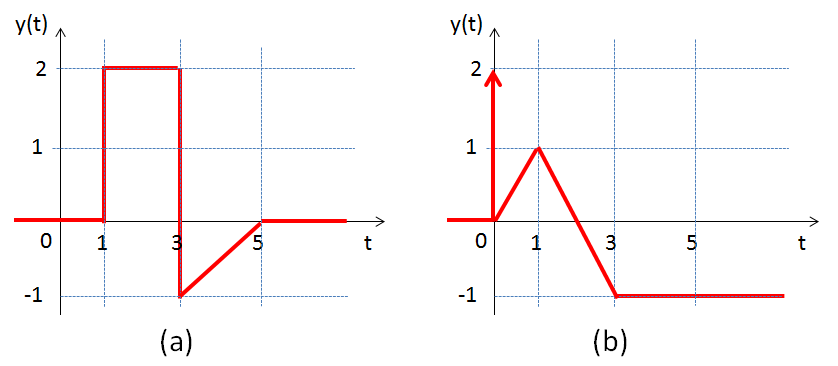
\includegraphics[scale=0.5]{images/Exo_2_2.jpg} 
 	\end{figure} \\
 
 	\vspace{0.5\baselineskip}
 	
 	2. Réécrivez sous la forme d'une fonction à valeurs réelles les fonctions suivantes et esquissez leur forme temporelle (pour t >0) :
 	
 	a. $x(t) = (1+j)e^{j\cdot 10t}$ 
 	
 	b. $y(t) = e^{(-2+j)t}\cdot u(t-2)$ 
 	
 	c. $z(t) = e^{(-1+2j)t}+e^{(-1-2j)t}$
 	
 	\vspace{1\baselineskip}	
 	
 	\textbf{\underline{Correction exercice 2}}\\
 	
 	1. a. $y(t)=2u(t-1)-3u(t-3)+(0.5t-2.5)(u(t-3)-u(t-5))$\\
 	
 	b. $y(t)=\delta(t)+t(u(t)-u(t-1))+(-t+2)(u(t-1)-u(t-3))$\\
 	
 	2. a. $x(t)=Re[(1+j)e^{-j10t}]=Re[\sqrt{2}e^{j\frac{\pi}{4}}e^{j10t}]=\sqrt{2}cos(10t+\frac{\pi}{4})$. Autre forme possible : $x(t)=cos(10t)-sin(10t)$\\
 
 	b. $y(t)=e^{-2t}cos(t)u(t-2)$\\
 	
 	c. $z(t)=2e^{-t}cos(2t)$\\
 	
 	\subsubsection{Exercice 3}
 	
 	On dispose de la réponse indicielle d'un système linéaire, qui est esquissée ci-dessous. Elle a une forme exponentielle croissante.\\
 	
 	\begin{figure}[h!]
 		\centering
 		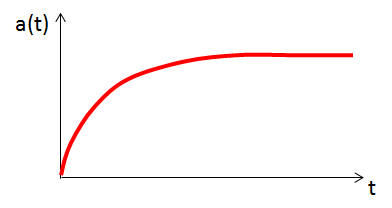
\includegraphics[scale=0.5]{images/Exo_2_3.png} 
 	\end{figure} 
 
 	Esquissez les réponses de ce système dans les cas suivants :\\
 	
 	a. l'excitation $e(t)=u(t)-u(t-1)$\\
 	
 	b. l'excitation $e(t)=t(u(t)-u(t-2))$\\
 	
 	c. l'excitation est la dérivée de celle utilisée pour obtenir la réponse indicielle.\\
 	
 	\subsubsection{Exercice 4}
 	
 	On excite un système linéaire à l'aide du signal suivant : $e(t)=e^{j2\pi t}$. La réponse obtenue, notée y(t), est égale à $y(t)=\frac{1}{2}e^{j(2\pi t+\frac{\pi}{3})}$.\\
 	
 	a. Réécrire la réponse sous la forme $y(t)=Acos(\omega t + \phi)$ et $y(t)=Bcos(\omega t)+Csin(\omega t)$, en précisant les valeurs de A, B, C et $\phi$.\\
 	
 	b. Donnez l'expression de la réponse du système lorsqu'il est excité par le signal ci-dessous.
 	
 	\begin{figure}[h!]
 		\centering
 		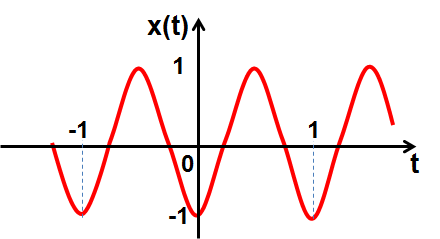
\includegraphics[scale=0.5]{images/Exo_2_4.png} 
 	\end{figure} 
 	
 	c. Calculez la réponse du système à l'excitation suivante : $x(t)=\frac{3\sqrt{3}}{2}cos(2\pi t)+\frac{1}{2}sin(2\pi t)$.\\
 	
 	
 	\textbf{\underline{Correction exercice 4}}\\
 	
 	a. $y(t)=\frac{1}{2}cos(2\pi t+\frac{\pi}{3})$ ou $y(t)=\frac{1}{4}cos(2\pi t)-\frac{\sqrt{3}}{2}sin(2\pi t)$. La pulsation du signal d'entrée est de $2\pi rad/s$ et sa fréquence 1 Hz. A cette fréquence, le signal atténue d'un facteur 2 l'amplitude du signal d'entrée et le retarde d'un angle de $\frac{\pi}{3}$.\\
 	
 	b. Le signal $x(t)=-cos(2\pi t)=cos(2\pi t+\pi)$. C'est aussi un signal de 1 Hz. On peut donc en déduire sa réponse : $y(t)=\frac{1}{2}cos(2\pi t+\frac{4\pi}{3})$.\\
 	
 	c. Le signal d'excitation peut se réécrire : $x(t)=3cos(2\pi t-\frac{\pi}{6})$. Sa fréquence est aussi égale à 1 Hz. Sa réponse est donc égale à : $\frac{3}{2}cos(2\pi t+\frac{\pi}{6})$.\\
 	
 	
 	
 
  	
 	\subsubsection{Exercice 5 - Réponse indicielle d'un circuit RC}
 	
 	On reprend le circuit RC dont on a étudié la réponse dans la partie VI.3. On considère deux cas : celui où le condensateur est déchargé initialement, puis celui où il est chargé. 
 	
 	a. Calculez la réponse naturelle du circuit lorsque le condensateur est initialement chargé.
 	
 	b. En déduire la réponse impulsionnelle du circuit.
 	
 	c. Calculez la réponse lorsque le circuit est soumis à un échelon de Heaviside d'amplitude E, dans les deux cas (charge initiale absente ou présente).
 	
 	d. En déduire la réponse indicielle du circuit.
 	 
 	\vspace{1\baselineskip}
 	
 	\subsubsection{Exercice 6}
 	
 	On considère les deux circuits électriques ci-dessous. Pour le circuit (a), la tension initiale (t=0) aux bornes du condensateur C est notée $U_{C0}$. Pour le circuit (b), un courant noté $I_L0$ traverse la bobine L. La sortie de ces deux circuits est la tension $U_{S}$.
 	
 	\begin{figure}[h!]
 		\centering
 		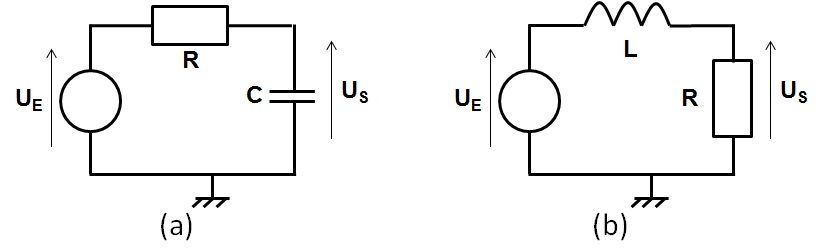
\includegraphics[scale=0.5]{images/Exo_2_4.jpg} 
 	\end{figure} 
 	
 	a. Déterminez les fréquences et les réponses naturelles de ces deux circuits. Quels sont les ordres de ces deux systèmes ? 
 	
 	b. On excite ces deux systèmes à l'aide d'un échelon de Heaviside d'amplitude notée E. Déterminez la réponse indicielle de ces deux circuits. 
 	
 	c. Déterminez les fonctions de transfert de ces deux circuits.
 	
 	\vspace{1\baselineskip}
 	
 	\subsubsection{Exercice 7 - Fonction de transfert d'un circuit résonant}
 	
 	On reprend le circuit RLC présenté dans la partie IV.4. Celui-ci est excité par un générateur de courant I, comme le montre la figure ci-dessous. On s'intéresse à la tension U aux bornes de ce circuit. On considère que la résistance R est grande et $R>>\sqrt{\frac{L}{C}}$.
 	 	
 	\begin{figure}[h!]
 		\centering
 		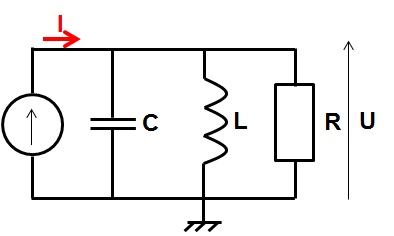
\includegraphics[scale=0.5]{images/Exo_2_5.jpg} 
 	\end{figure} 
 
 	a. Déterminez la fonction de transfert de ce circuit. La mettre sous la forme $\frac{Gp}{p^2+2\alpha p+\omega_{0}^{2}}$.\\
 	
 	b. Précisez l'unité de la fonction de transfert. \\
 	
 	c. Ce circuit est-il stable ?\\
 	
 	d. On considère maintenant que le terme $\alpha$ est négligeable et une excitation cosinusoïdale du circuit. Y a t-il une fréquence particulière où la réponse présente un maximum ? Si oui, laquelle ? \\
 	
 	e. Donnez l'expression de la réponse temporelle du circuit en régime permanent.\\
 	
 	\textbf{\underline{Correction exercice 7}}\\
 	
 	a. On peut établir l'équation différentielle du circuit en remarquant que :
 	\begin{itemize}
 		\item $i=i_R+i_L+i_C$, où $i_R$ est le courant traversant la résistance, $i_L$ celui traversant l'inductance et $i_C$ celui traversant le condensateur
 		\item $U=r.i_R$, $i_L=\frac{1}{L}\int U dt$ et $i_C=C\frac{dU}{dt}$
 	\end{itemize} 
 	
 	\begin{equation*}
 	\frac{U}{R}+\frac{1}{L}\int i_L dt+C\frac{dU}{dt}=i
 	\end{equation*}
 	
 	La fonction de transfert suppose que l'excitation est de type exponentiel complexe : $i=\hat{I}e^{pt}$, donc la réponse est aussi de type exponentiel complexe : $U=\hat{U}e^{pt}$ :
 	\begin{equation*}
 	\frac{\hat{U}e^{pt}}{R}+\frac{1}{L}\int \hat{U}e^{pt} dt+C\frac{d(\hat{U}e^{pt})}{dt}=\hat{I}e^{pt}
 	\end{equation*}
 	\begin{equation*}
 	\frac{\hat{U}e^{pt}}{R}+\frac{1}{Lp}\hat{U}e^{pt}+Cp\hat{U}e^{pt}=\hat{I}e^{pt}
 	\end{equation*}
 	\begin{equation*}
 	\frac{\hat{U}}{\hat{I}}=\frac{RLp}{R+Lp+RLCp^2}=\frac{1}{C}\frac{p}{p^2+\frac{1}{RC}p+\frac{1}{LC}}
 	\end{equation*}
 	
 	On trouve donc la forme indiquée avec $G=\frac{1}{C}$, $\alpha=\frac{1}{2RC}$ et $\omega_0^2=\frac{1}{LC}$.\\
 	
 	b. Rapport entre tension et courant, donc une impédance (ohms).\\
 	
 	c. Etude des racines du dénominateur. Ordre 2 , deux pôles.
 	Déterminant : $\Delta=4(\alpha^2-\omega_{0}^2$). Comme R est très grand, le dénominateur est négatif. Les deux pôles sont complexes et conjugués et s'écrivent :
 	\begin{equation*}
 	p_1=-\alpha+j\sqrt{\omega_{0}^2-\alpha^2}~~~et~~~p_2=-\alpha-j\sqrt{\omega_{0}^2-\alpha^2}
 	\end{equation*}
 	
 	La partie réelle des pôles étant négative, le système est stable. La partie imaginaire entrainant un comportement oscillant. \\
 	
 	d. Si $\alpha$ est négligeable, les pôles sont purement imaginaires. La fonction de transfert s'écrit alors :
 	\begin{equation*}
 	\frac{\hat{U}}{\hat{I}}=\frac{1}{C}\frac{p}{p^2+\omega_0^2}
 	\end{equation*}
 	Si l'excitation est cosinusoïdale, cela signifie que : $p = j\omega$ où $\omega$ est la pulsation de l'excitation. Si $\omega=\omega_0$, le rapport entre U et I devient infini. Cette fréquence est appelée fréquence de résonance.\\
 	
 	e. En posant $i=\hat{I}e^{pt}$, on peut déterminer l'amplitude complexe de la tension U : 
 	\begin{equation*}
 	\hat(U)=\frac{1}{C}\frac{p}{p^2+\omega_0^2}
 	\end{equation*}
 	Dans le cas d'une excitation cosinusoïdale : $u(t)=\hat(U)e^{j\omega t}$ avec :
 	\begin{equation*}
 	\hat(U)=\frac{1}{C}\frac{j\omega}{-\omega^2+\omega_0^2}
 	\end{equation*}
 	L'expression de la tension s'écrit donc :
 	\begin{equation*}
 	u(t)=Re[\frac{1}{C}\frac{j\omega}{-\omega^2+\omega_0^2}e^{j\omega t}]=\frac{\omega}{C(-\omega^2+\omega_0^2)}cos(\omega t+\frac{\pi}{2})
 	\end{equation*}
 	
 	
 	
 	
 	
 	\subsubsection{Exercice 8}
 	
 	On considère le système dont le fonctionnement est décrit par le schéma-bloc ci-dessous. Celui-ci transforme un signal d'entrée e(t) et délivre en sortie un signal s(t). 
 	
 	\begin{figure}[h!]
 		\centering
 		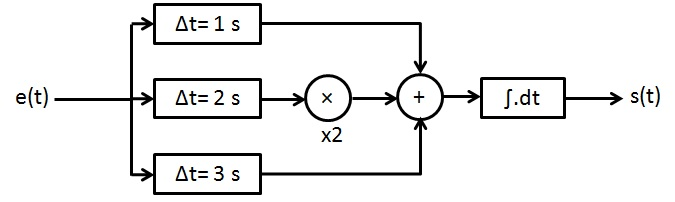
\includegraphics[scale=0.5]{images/Exo_2_6.jpg} 
 	\end{figure}
 
 	a. Le système est-il linéaire, à temps invariant, causal ?
 	
 	b. Ecrire l'équation différentielle générale de ce système.
 	
 	c. Déterminez l'expression de la réponse impulsionnelle h(t) du système. Esquissez l'allure temporelle de la réponse impulsionnelle. 
 	
 	d. Déterminez l'expression de la fonction de transfert H(p) du système. Précisez les pôles de la fonction de transfert. Que concluez-vous sur sa stabilité ?
 
 	\vspace{1\baselineskip}
 	
 		\textbf{\underline{Correction exercice 8}}\\
 	a. Le système transforme le signal d'entrée à partir de trois opérations de base : retard, multiplication par une constante et intégration temporelle. Il s'agit d'opérations purement linéaires. Le fonctionnement du système est indépendant du temps. Il s'agit donc d'un système LTI. De plus, il est causal puisque la sortie ne dépend que des états passés du signal d'entrée.\\
 	
 	b. $s(t)=\int e(t-1)+2e(t-2)+e(t-3) dt$. Cette équation intégrale peut être réécrite sous une forme différentielle : $\frac{ds}{dt}=e(t-1)+2e(t-2)+e(t-3)$ 
 	
 	c. On considère une entrée égale à une impulsion de Dirac : $e(t) = \delta(t)$.	Avant l'intégrateur, le signal résultant s'écrit : $e(t-1)+2e(t-2)+e(t-3)=\delta(t-1)+2\delta(t-2)+\delta(t-3)$. L'impulsion de Dirac résultant de la dérivée de l'échelon de Heaviside, après intégration, la sortie du système est donnée par : $s(t) = h(t) = u(t-1)+2u(t-2)+u(t-3)$.\\
 	
 	d. Le calcul de la fonction de transfert suppose une excitation de type exponentielle complexe : $e(t)=\hat{E}e^{pt}$, où $\hat{E}$ est l'amplitude complexe du signal d'entrée. Le système étant linéaire, la réponse a aussi une forme d'exponentielle complexe. Elle s'écrit donc : $s(t)=\hat{S}e^{pt}$. L'effet du système ne modifie que l'amplitude complexe ou phaseur.
 	
 	En repartant de l'équation différentielle générale du système : $\frac{ds}{dt}=\frac{d}{dt}\hat{S}e^{pt}=p\hat{S}e^{pt}$. L'effet d'un retard se détermine facilement : $e(t-1)=\hat{E}e^{p(t-1)}=\hat{E}e^{-p}e^{pt}$. L'équation différentielle se réécrit donc :
 	
 	\begin{equation*}
 	p\hat{S}e^{pt}=\hat{E}e^{-p}e^{pt}+2\hat{E}e^{-2p}e^{pt}+\hat{E}e^{-3p}e^{pt}
 	\end{equation*}
 	\begin{equation*}
 	\frac{\hat{S}}{\hat{E}}=\frac{e^{-p}(1+2e^{-p}+e^{-2p})}{p}
 	\end{equation*}
 	
 	La fonction de transfert ne présente un pôle nul.  Il est lié à l'effet intégrateur pur du système. Le système est en limite de stabilité. Un intégrateur pur est en effet instable en pratique. La moindre excitation avec une moyenne non nulle est capable de faire diverger la sortie.
 	
 	
	
	\newpage
	
	\chapter{Transformée de Laplace}
	
	
	\subsubsection{Exercice 1}
	
	Déterminez les transformées de Laplace des fonctions suivantes :
	
	a. $x(t)=e^{-2t}u(t-1)$
	
	b. $y(t)=e^{-2(t-1)}u(t-1)$
	
	c. $z(t) = \sqrt{2}cos(t+\frac{\pi}{4})$
	
	\begin{figure}[h!]
		\centering
		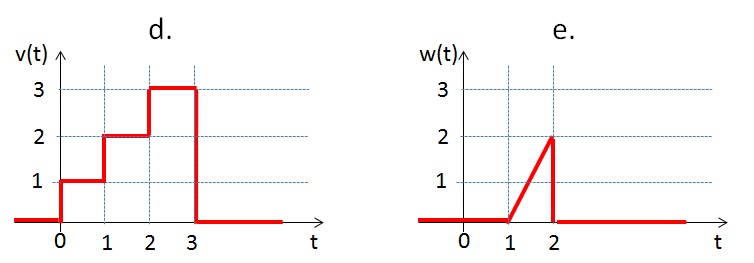
\includegraphics[scale=0.5]{images/Exo_2_1_a.jpg} 
	\end{figure} 

	\begin{figure}[h!]
		\centering
		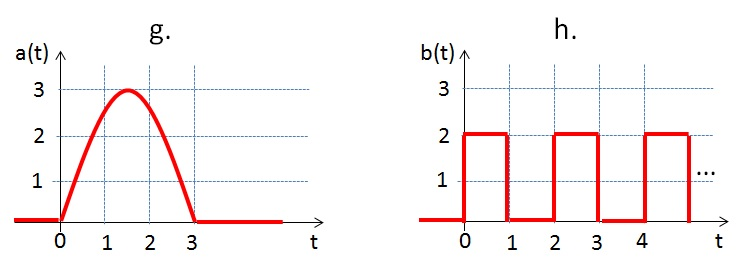
\includegraphics[scale=0.5]{images/Exo_2_1_b.jpg} 
	\end{figure}
	
	
	
	\vspace{1\baselineskip}
	
	\textbf{\underline{Correction exercice 1}}\\
	a. Attention à ne pas utiliser le théorème du retard trop hâtivement (seul l'échelon de Heaviside est retardé) !
	
	$X(p) = \int_{0}^{+\infty} e^{-2t}u(t-1)e^{-pt}dt=\int_{1}^{+\infty} e^{-(p+2)t}dt=\frac{e^{-(p+2)}}{p+2}$
	
	\vspace{0.5\baselineskip}
	
	b. Théorème du retard : $Y(p) = \frac{e^{-p}}{p+2}$
	
	\vspace{0.5\baselineskip}
	
	c. $z(t) = \sqrt{2}(cos(t)cos(\frac{\pi}{4})-sin(t)sin(\frac{\pi}{4}))=cos(t)-sin(t)$
	
	$Z(p) = \frac{p}{p^{2}+1}-\frac{1}{p^{2}+1}=\frac{p-1}{p^{2}+1}$
	
	\vspace{0.5\baselineskip}
	
	d. $v(t) = u(t)+u(t-1)+u(t-2)-3u(t-3)~\Rightarrow~V(p)=\frac{1+e^{-p}+e^{-2p}-3e^{-3p}}{p}$ 
	
	\vspace{0.5\baselineskip}
	
	e. $w(t) = 2(t-1)u(t-1)-2(t-2)u(t-2)-2u(t-2)~\Rightarrow~W(p)=\frac{2e^{-p}}{p^{2}}(1-e^{-p}-pe^{-p})$ 
	
	\vspace{0.5\baselineskip}
	
	g. $a(t)=3sin(\frac{\pi}{3}t)u(t)+3sin(\frac{\pi}{3}(t-3))u(t-3)~\Rightarrow~A(p)=\frac{\pi(1+e^{-3p})}{p^{2}+(\frac{\pi}{3})^{2}}$
	
	\vspace{0.5\baselineskip}
	
	h. Il s'agit d'une fonction périodique. En déterminant la transformée de Laplace de la fonction génératrice $B_{0}(p)$, on pourra déterminer ensuite celle de la fonction périodique $B(p)$.
	
	$b_{0}(t)=2u(t)-2u(t-1)~\Rightarrow~B_{0}(p)=2\frac{1-e^{-p}}{p}$
	
	La périodicité d'une fonction de période T se traduit, dans le domaine de Laplace par une multiplication par le terme : $\frac{1}{1-e^{pT}}$. La transformée de Laplace de la fonction b(t), de période T = 2, s'écrit donc : $B(p) =2\frac{1-e^{-p}}{p(1-e^{2p})} $.
	
	\vspace{0.5\baselineskip}
	
	
	\subsubsection{Exercice 2}
	
	Déterminez les expressions temporelles des fonctions suivantes :
	
	a. $X(p)=\frac{p-4}{p^{2}+16}$ 
	
	b. $Y(p) = \frac{p^{2}+3p+3-\frac{6}{p}}{p^{2}}$ 
	
	c. $Z(p) = \frac{p^{2}+4p+4}{p^{2}+2p+2}$
	
	d. $W(p) = \frac{p-1+e^{-p}}{p^{2}(1-e^{-p})}$. Tracez cette fonction.
	
	
	\vspace{1\baselineskip}
	
	\textbf{\underline{Correction exercice 2}}\\
	
	a. $x(t)=[cos(4t)-sin(4t)]u(t)$
	
	b. $Y(p)=1+\frac{3}{p}+\frac{3}{p^{2}}-\frac{6}{p^{3}} ~~\Longrightarrow~ y(t)=\delta(t)+3u(t)+3t\cdot u(t)-6t^{2}\cdot u(t)$
	
	c. $Z(p)=1+\frac{2p+2}{p^{2}+2p+2}~~\Longrightarrow~z(t)=\delta(t)+2e^{-t}cos(t)u(t)$
	
	d. Laissons d'abord de côté le terme $\frac{1}{1-e^{-p}}$ car il indique une périodicité de période T=1. Soit la fonction $W_{1}(p)= \frac{p-1+e^{-p}}{p^{2}}=\frac{1}{p}-\frac{1}{p^{2}}+\frac{e^{-p}}{p^{2}}$. On en déduit $w_{1}(t)=u(t)-tu(t)+(t-1)u(t)$ (pour le dernier terme, utilisation du théorème du retard). La fonction $w(t) =w_{1}(t-kT)$, avec k > 0. Cela correspond à une fonction périodique en dent de scie.
	
	
	\vspace{1\baselineskip}
	
	\subsubsection{Exercice 3}
	
	Résoudre les équation différentielles suivantes :
	
	a. $x"+2x'+x=e^{-t}u(t)$, avec x(0) = 0 et x'(0) = 0. 
	
	b. $x"+6x'+8x=\delta(t)$ avec x(0)=1 et x'(0)=3. 
	
	\vspace{1\baselineskip}
	
	\textbf{\underline{Correction exercice 3}}\\
	
	a. $p^{2}X(p)+2pX(p)+X(p)=\frac{1}{p+1}~\Rightarrow X(p)=\frac{1}{(p+1)^{3}}$. En considérant le théorème de translation de p, en posant P=p+1 : $X(P)=\frac{1}{P^{3}}$, soit $X(t)=t^{2}u(t)$, qui devient après changement de variable : $x(t)=e^{-t}t^{2}u(t)$.
	
	b. $X(p)=\frac{p+10}{(p+2)(p+4)} = \frac{4}{p+2}-\frac{3}{p+4}$, d'où $x(t) = (4e^{-2t}-3e^{-4t})u(t)$.
	
	\vspace{1\baselineskip}
	
	
	\subsubsection{Exercice 4}
	
	On reprend l'exercice 8 du chapitre 2.
	
	
	\begin{figure}[h!]
		\centering
		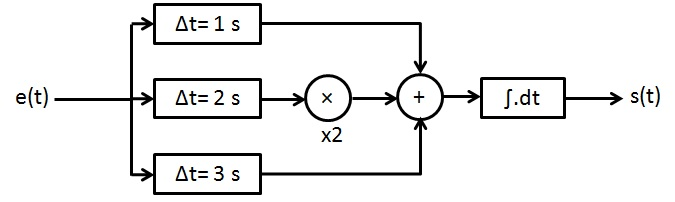
\includegraphics[scale=0.5]{images/Exo_2_6.jpg} 
	\end{figure}
	
	a. Ecrivez la fonction de transfert du système dans le domaine de Laplace.
	
	b. Calculez la réponse indicielle du système. On supposera que les conditions initiales de tous les nœuds internes du système sont nulles. 
	
	\vspace{1\baselineskip}
	
	\textbf{\underline{Correction exercice 4}}\\
	
	a. \begin{equation*}
	H(p)=\frac{S(p)}{E(p)}=\frac{e^{-p}+2e^{-2p}+e^{-3p}}{p}
	\end{equation*}
	
	b. Soit $e(t)=u(t)~\Rightarrow~E(p)=\frac{1}{p}$. La transformée de Laplace du signal de sortie s'écrit donc :
	\begin{equation*}
	S(p)=H(p)E(p)=frac{e^{-p}+2e^{-2p}+e^{-3p}}{p^2}
	\end{equation*}
	On identifie une somme de terme en $\frac{1}{p^2}$ représentant des fonctions rampes, démarrant à 0 (pas de conditions initiales). Les termes exponentielles complexes introduisent des retards :
	\begin{equation*}
	s(t)=\mathcal{L}^{-1}=tu(t-1)+2tu(t-2)+tu(t-3)
	\end{equation*}
	
	Le signal en sortie diverge, à cause du caractère intégrateur du système.
	
	
	\vspace{1\baselineskip}
	
		
	\subsubsection{Exercice 5}
	
	On considère un circuit électrique, dont le courant i(t) est donné par l'équation ci-dessous.
	\begin{equation*}
		e(t)=\frac{d^{2}i}{dt^{2}}+7\frac{di}{dt}+10i(t)
	\end{equation*}
	On considère l'excitation suivante $e(t)=6e^{-3t}u(t)$. Les conditions initiales du circuit sont : $i(0) = 3~A$ et $\frac{di}{dt}(0)=3~A/s$.
	
	
	a. Etablir l'expression du courant dans le domaine de Laplace.
	
	b. En déduire l'expression temporelle du courant i(t).
	
	c. Vérifiez, en utilisant les expressions du courant dans le domaine de Laplace, puis dans le domaine temporel, que la condition initiale du courant est respectée. Déterminez ensuite les conditions finales.
	
	\vspace{1\baselineskip}
	
	\textbf{\underline{Correction exercice 5}}\\
	a. A partir de l'équation différentielle et des conditions initiales, la transformée de Laplace est la suivante :
	
	\begin{equation*}
		p^{2}I(p)-pi(0)-i(0)+7pI(p)-7i(0)+10I(p)=\frac{6}{p+3}
	\end{equation*}
	On transforme ensuite cette relation pour exprimer I(p) sous la forme d'une somme d'éléments dont nous disposons l'expression temporelle (par exemple, fonction rationnelle).
	\begin{equation*}
	I(p)\cdot (p^{2}+7p+10)=\frac{6}{p+3}+3(p+8)
	\end{equation*}
	\begin{equation*}
	I(p)\cdot (p+2)(p+5)=\frac{3(p^{2}+11p+26)}{p+3}
	\end{equation*}
	\begin{equation*}
	I(p)=\frac{3(p^{2}+11p+26)}{(p+3)(p+2)(p+5)}
	\end{equation*}
	En utilisant la méthode du cache, on décompose en pôles et résidus l'expression précédente.
	\begin{equation*}
		I(p)=\frac{A}{p+2}+\frac{B}{p+3}+\frac{C}{p+5}
	\end{equation*}
	\begin{equation*}
		(p+2)I(p)=\frac{3(p^{2}+11p+26)}{(p+3)(p+5)}=A+\frac{B(p+2)}{p+3}+\frac{C(p+2)}{p+5}~\rightarrow~p=-2~:~A=\frac{3((-2)^{2}+11\cdot (-2)+26)}{(-2+3)(-2+5)}=8
	\end{equation*}
	\begin{equation*}
	(p+3)I(p)=\frac{3(p^{2}+11p+26)}{(p+2)(p+5)}=\frac{A(p+3)}{p+2}+B+\frac{C(p+3)}{p+5}~\rightarrow~p=-3~:~B=\frac{3((-3)^{2}+11\cdot (-3)+26)}{(-3+2)(-3+5)}=-3
	\end{equation*}
	\begin{equation*}
	(p+5)I(p)=\frac{3(p^{2}+11p+26)}{(p+2)(p+3)}=\frac{A(p+5)}{p+2}+\frac{B(p+5)}{p+3}+C~\rightarrow~p=-5~:~C=\frac{3((-5)^{2}+11\cdot (-5)+26)}{(-5+2)(-5+3)}=-2
	\end{equation*}
	L'expression du courant dans le domaine de Laplace peut s'écrire de la manière suivante :
	\begin{equation*}
		I(p)=\frac{8}{p+2}-\frac{3}{p+3}-\frac{2}{p+5}
	\end{equation*}
	
	\vspace{0.5\baselineskip}
	
	b. A partir de l'expression précédente, on en déduit directement la forme temporelle du courant à l'aide de la table des transformées de Laplace inverse usuelles.
	\begin{equation*}
	i(t)=(8e^{-2t}-3e^{-3t}-2e^{-5t})u(t)
	\end{equation*}
	
	\vspace{0.5\baselineskip}
	
	c. Condition initiale du courant : d'après les propriétés de la transformée de Laplace, on sait que :
	\begin{equation*}
		\lim_{t\rightarrow0^{+}} i(t)=\lim_{p \to +\infty} pI(p)
	\end{equation*}
	On vérifie cette égalité en retrouvant la valeur de la condition initiale du courant.
	\begin{equation*}
		\lim_{t\rightarrow0^{+}} i(t)=\lim_{t\rightarrow0^{+}}(8e^{-2t}-3e^{-3t}-2e^{-5t})u(t)=8-3-2=3~A
	\end{equation*}
	\begin{equation*}
		\lim_{p \to +\infty} pI(p)=	\lim_{p \to +\infty} \frac{8p}{p+2}-\frac{3p}{p+3}-\frac{2p}{p+5}=8-3-2=3~A
	\end{equation*}
	
	Condition finale du courant : d'après les propriétés de la transformée de Laplace, on doit vérifier que :
	\begin{equation*}
	\lim_{t \to +\infty} i(t)=\lim_{p \to 0} pI(p)
	\end{equation*}
	
	On détermine ainsi la valeur finale du courant.
	\begin{equation*}
	\lim_{t \to +\infty} i(t)=\lim_{t \to +\infty}(8e^{-2t}-3e^{-3t}-2e^{-5t})u(t)=0~A
	\end{equation*}
	\begin{equation*}
	\lim_{p \to 0} pI(p)=	\lim_{p \to 0} \frac{8p}{p+2}-\frac{3p}{p+3}-\frac{2p}{p+5}=0~A
	\end{equation*}
	
	\vspace{1\baselineskip}
	
	
	\subsubsection{Exercice 6 - Réponse d'un moteur à courant continu à aimants permanents}

	Le fonctionnement d'un moteur est gouverné par un modèle électromécanique, se présentant sous la forme de plusieurs équations différentielles reliant grandeurs électriques et mécaniques. Dans cet exercice, nous allons étudier le modèle simplifié d'un moteur à courant continu à aimants permanents. La figure ci-dessous présente le modèle électrique équivalent de l'induit. Celui-ci est modélisé par un circuit RL et est excité par une tension de commande notée $U_{C}$. Lorsque le moteur tourne, une force contre électromotrice (fcem) E est induite, qui est proportionnelle à la vitesse angulaire du moteur $\Omega$. 
	\begin{figure}[h!]
		\centering
		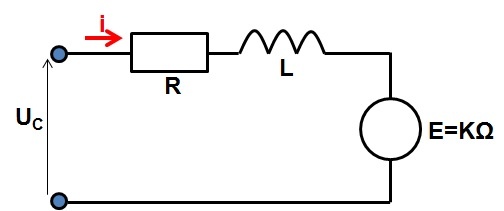
\includegraphics[scale=0.5]{images/Exo3_moteur.jpg} 
	\end{figure}	
	Le courant i circulant dans l'induit produit un couple moteur $C_{m}$, selon la même constante de proportionnalité K que celle liant la fcem et la vitesse de rotation du moteur. A ce couple moteur s'opposent plusieurs sources de couples résistants $C_{R}$ :
	\begin{itemize}
		\item l'inertie du moteur, donnée par le moment d'inertie J
		\item les frottements visqueux, caractérisés par le coefficient de frottement visqueux f
	\end{itemize}
	L'équation mécanique du moteur s'écrit alors :
	\begin{equation*}
		C_{m} = C_{R} = J\frac{d\Omega}{dt}+f\Omega
	\end{equation*}	
	Nous cherchons à déterminer la vitesse de rotation du moteur en fonction de l'excitation appliquée.
	Dans cet exercice, on considèrera les valeurs suivantes : r=0.2 $\Omega$, L = 0.2 mH, K = 0.057 N.m/A, J = $650.10^{-7}~kg.m^{2}$, f = $2.3.10^{-5}~N.m/rad.s^{-1}$. On suppose que le moteur est initialement à l'arrêt.\\
	
	
	a. Etablir l'équation différentielle reliant la vitesse de rotation et l'excitation $U_{C}$ du moteur.
	
	b. Déterminez la fonction de transfert du moteur dans le domaine de Laplace. Exprimez-la sous la forme $\frac{G}{p^{2}+2\alpha p+\omega_{0}^{2}}$. Précisez les expressions littérales de G, $\alpha$ et $\omega_{0}$. Calculez leurs valeurs.
	
	c. Calculez les pôles du système. Que concluez-vous sur la réponse du système ? Est-ce satisfaisant ?
	
	d. Déterminez l'expression de la réponse impulsionnelle du système. Esquissez son profil temporel.
	
	e. Question bonus : En t = 0, on applique une commande de type échelon unitaire d'amplitude $Uc_{0}$ = 10 V. Déterminez l'expression de l'évolution de la vitesse angulaire. Esquissez le profil temporel de la vitesse angulaire. En régime permanent, quelle est la valeur de la vitesse ? 
	
	\vspace{1\baselineskip}
	
	\textbf{\underline{Correction exercice 6}}\\
	a. Relation électrique et en remplaçant le courant par le couple :
	\begin{equation*}
	U_C(t) = L\frac{di}{dt}+ri+E=L\frac{di}{dt}+ri+K\Omega(t)
	\end{equation*}
	\begin{equation*}
	U_C(t) =\frac{L}{K}\frac{dC_m}{dt}+\frac{r}{K}C_m+K\Omega(t)
	\end{equation*}
	
	En utilisant l'équation mécanique :
	\begin{equation*}
	U_C(t) =\frac{L}{K}\frac{d}{dt}(J\frac{d\Omega}{dt}+f\Omega)+\frac{r}{K}(J\frac{d\Omega}{dt}+f\Omega)+K\Omega(t)
	\end{equation*}
	\begin{equation*}
	U_C(t) =\frac{LJ}{K}\frac{d^2\Omega}{dt^2}+\frac{Lf+rJ}{K}\frac{d\Omega}{dt}+\frac{rf+K^2}{K}\Omega(t)
	\end{equation*}
	
	b. Passage dans le domaine de Laplace :
	\begin{equation*}
	U_C(p) =\frac{LJ}{K}p^2\Omega(p)+\frac{Lf+rJ}{K}p\Omega(p)+\frac{rf+K^2}{K}\Omega(p)
	\end{equation*}
	La fonction de transfert du moteur relie la tension de commande (l'excitation) à la vitesse de rotation (la réponse) :
	\begin{equation*}
	H(p)=\frac{\Omega(p)}{U_C(p)}=\frac{\frac{K}{LJ}}{p^2+(\frac{f}{J}+\frac{r}{L})p+\frac{rf+K^2}{LJ}}
	\end{equation*}
	On retrouve la fonction de transfert typique d'un système d'ordre 2, que l'on peut écrire sous cette forme :
	\begin{equation*}
	H(p)=\frac{G}{p^{2}+2\alpha p+\omega_{0}^{2}}
	\end{equation*}
	avec  : $G=\frac{K}{LJ}=4384615$, $\alpha=0.5(\frac{f}{J}+\frac{r}{L})=500.18$ et $\omega_{0}=\sqrt{\frac{rf+K^2}{LJ}}=500.28$.\\
	
	c. Les pôles sont les racines du polynôme $p^{2}+2\alpha p+\omega_{0}^{2}$. Son déterminant vaut : $\Delta=4(\alpha^2-\omega_{0}^2)$. Il est négatif donc les deux racines sont complexes, conjuguées et égales à :
	\begin{equation*}
	p_1 =-\alpha+j\sqrt{\omega_{0}^2-\alpha^2}~~~et~~~	p_2 =-\alpha-j\sqrt{\omega_{0}^2-\alpha^2}
	\end{equation*}
	Le systèmes présentent deux pôles complexes, dont les parties réelles sont négatives. Le système est donc stable. La partie imaginaire introduit un comportement oscillant, mais qui reste limité en raison de la faiblesse de la partie imaginaire. Lorsque le moteur sera excité, sa réponse sera gouvernée par un comportement exponentiel décroissant. Cette stabilité et l'absence d'oscillations sont deux propriétés attendues pour le contrôle d'un moteur, afin d'éviter tout à-coup et instabilité. De plus, en éliminant toute oscillation, le système se stabilise rapidement en régime permanent (vitesse finale atteinte rapidement).\\ 
	
	d. La réponse impulsionnelle est directement la transformée de Laplace inverse de la fonction de transfert, que l'on décompose d'abord en fractions partielles. On peut montrer que :
	\begin{equation*}
	\frac{1}{p^{2}+2\alpha p+\omega_{0}^{2}}=\frac{A}{p-p_1}+\frac{B}{p-p_2}=\frac{j}{2\sqrt(\omega_{0}^2-\alpha^2)}(\frac{-1}{p-p_1}+\frac{1}{p-p_2})
	\end{equation*}
	On décompose donc la fonction de transfert sous la forme suivante :
	\begin{equation*}
	H(p)=\frac{jG}{2\sqrt(\omega_{0}^2-\alpha^2)}(\frac{-1}{p-p_1}+\frac{1}{p-p_2})
	\end{equation*}
	
	En identifiant la transformée de Laplace inverse des fractions partielles (exponentielle complexe), on trouve la réponse impulsionnelle h(t) :
	\begin{equation*}
	h(t)=\mathcal{L}^{-1}=\frac{jG}{2\sqrt(\omega_{0}^2-\alpha^2)}e^{-\alpha t}(-e^{j\sqrt{\omega_{0}^2-\alpha^2}t}+e^{-j\sqrt{\omega_{0}^2-\alpha^2}t})
	\end{equation*}
	\begin{equation*}
	h(t)=\frac{G}{\sqrt(\omega_{0}^2-\alpha^2)}e^{-\alpha t}sin(\sqrt{\omega_{0}^2-\alpha^2}t)
	\end{equation*}
	
	La figure ci-dessous présente un tracé de la réponse impulsionnelle :
	
	\begin{figure}[h!]
		\centering
		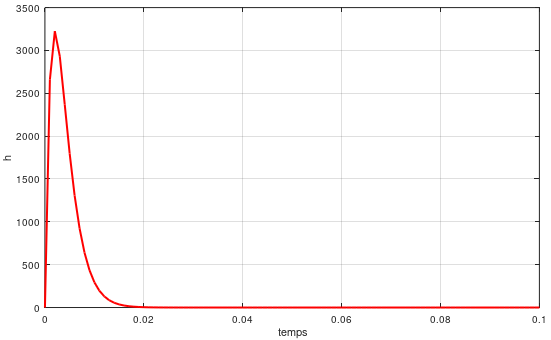
\includegraphics[scale=0.7]{images/reponse_impuls_moteur.png} 
	\end{figure}
	
	
	e. Le calcul de la réponse indicielle a(t) peut se faire directement à partir de la réponse impulsionnelle, en l'intégrant de 0 à t.
	\begin{equation*}
	a(t)=\int_{0}^{t}h(\tau)d\tau=\frac{jG}{2\sqrt(\omega_{0}^2-\alpha^2)}\int_{0}^{t}(-e^{j\sqrt{\omega_{0}^2-\alpha^2}t}+e^{-j\sqrt{\omega_{0}^2-\alpha^2}t})d\tau
	\end{equation*}
	On arrive au résultat final suivant :
	\begin{equation*}
	a(t)\frac{G}{\omega_{0}^2}(1-e^{-\alpha t}cos(\sqrt{\omega_{0}^2-\alpha^2}t)-\frac{\alpha}{\sqrt{\omega_{0}^2-\alpha^2}}e^{-\alpha t}sin(\sqrt{\omega_{0}^2-\alpha^2}t))
	\end{equation*}
	
	La réponse est illustrée ci-dessous (pour un indice d'amplitude = 10 V). Il est la superposition d'un terme exponentiel décroissant et de terme trigonométriques, avec des oscillations de pulsation égale à $\sqrt{\omega_{0}^2-\alpha^2}$. Les termes $\alpha^2$ et $\omega_{0}^2$ étant très proches, les oscillations sont de très grande période et n'ont pas d'effets visibles.
	
	\begin{figure}[h!]
		\centering
		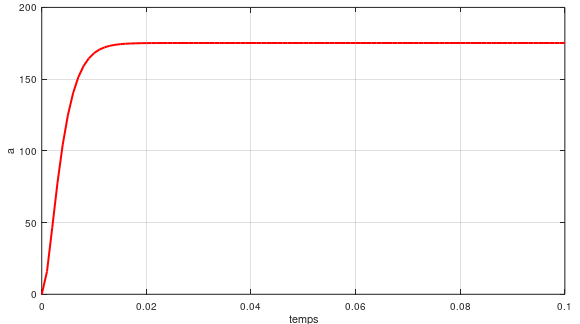
\includegraphics[scale=0.7]{images/reponse_indice_moteur.png} 
	\end{figure}

	En régime permanent, pour un échelon de 10 V, la valeur de la vitesse de rotation est égale à $10\frac{G}{\omega_{0}^2}=175 rad.s^{-1}$.\\
	
	
	
	
	
	
	\newpage
	
	\chapter{Filtrage}
	
	\subsubsection{Exercice 1}
	Soit les fonctions de transfert suivantes (en fonction de la fréquence). Esquissez le diagramme de Bode (asymptotique). \\
	
	a. $G(\omega)=\frac{j10\omega}{(1+j\frac{\omega}{628})(1+j\frac{\omega}{6280})(1+j\frac{\omega}{31400})}$\\
	
	b. $H(p)=\frac{p^3+4p^2+4p}{p^2+60p+800}$\\
	
	c. $Z(p)=\frac{p+10}{p(p+100)}$\\

	
	\subsubsection{Exercice 2 - Circuit bouchon}
	On considère le filtre décrit ci-dessous.
	
	\begin{figure}[h!]
		\centering
		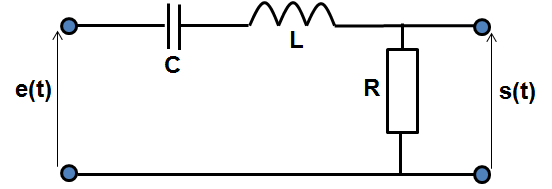
\includegraphics[scale=0.5]{images/circuit_bouchon.png} 
	\end{figure}

	1. Etablir la fonction de transfert $H(\omega)$ de ce filtre. On la mettra sous la forme : $H(\omega)=\frac{2\alpha \omega}{2\alpha \omega+j(\omega^{2}-\omega_{0}^{2})}$. Précisez la signification des termes $\alpha$ et $\omega_{0}$.\\
	
	2. Tracez 'évolution de la fonction de transfert de ce filtre en fonction de la fréquence. Précisez l'amplitude maximale et les fréquences caractéristiques. Quelle est la nature du filtre ? Son ordre ?\\
	
	3. Déterminez la bande passante à 3 dB de ce filtre. \\
	
	4. Déterminez le facteur de qualité de ce filtre. \\
	
	5. On fixe L = $100 \mu H$. On souhaite réaliser un filtre centré sur 200 kHz avec une bande passante de 10 kHz. Proposez des valeurs pour R et C.
	
	\vspace{1\baselineskip}
	
	\textbf{\underline{Correction exercice 2}}\\
	
	1. $H(p)=\frac{R}{R+Lp+\frac{1}{Cp}}=\frac{\frac{R}{L}p}{p^{2}+\frac{R}{L}p+\frac{1}{LC}} = \frac{2\alpha p}{p^{2}+2\alpha p+\omega_{0}^{2}}$, avec $\alpha=\frac{R}{2L}$ et $\omega_{0}^{2}=\frac{1}{LC}$. Le terme $\alpha$ est le coefficient d'amortissement du filtre, $\omega_{0}$ sa pulsation de résonance.
	
	En régime harmonique, la fonction de transfert devient :
	\begin{equation*}
	H(\omega)=\frac{2\alpha \omega}{2\alpha \omega+j(\omega^{2}-\omega_{0}^{2})}
	\end{equation*} 
	
	2. Tracé du diagramme de Bode :
	
	\begin{figure}[h!]
		\centering
		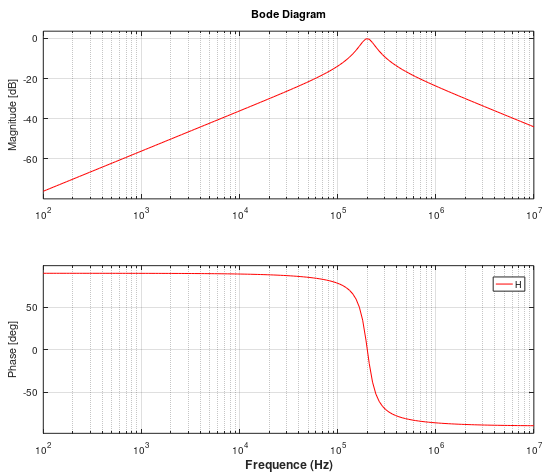
\includegraphics[scale=0.5]{images/Bode_circuit_bouchon.png} 
	\end{figure}

	Il s'agit d'un filtre passe-bande d'ordre 2. La fréquence $f=\frac{1}{2\pi \sqrt(LC)}$ est une fréquence de résonance pour laquelle il n'y a pas d'atténuation.\\
	
	3. La bande passante est délimitée par deux pulsation $\omega_{m}$ et $\omega_{p}$, avec $\omega_{p} > \omega_{0} > \omega_{m}$. A ces fréquences, on a :
	\begin{equation*}
	|H(\omega)|^{2}=\frac{1}{2}~\Rightarrow~\frac{4\alpha^{2} \omega^{2}}{4\alpha^{2} \omega^{2}+(\omega^{2}-\omega_{0}^{2})^{2}}=\frac{1}{2}
	\end{equation*}
	On doit résoudre l'équation : $(\omega^{2}-\omega_{0}^{2})^{2}=4\alpha^{2} \omega^{2}$.
	
	Commençons par la pulsation $\omega_{p}$ : $\omega_{p}^{2}-\omega_{0}^{2}=2\alpha \omega_{p}$. On doit résoudre l'équation du second ordre :
	\begin{equation*}
	\omega_{p}^{2}-2\alpha \omega_{p}-\omega_{0}^{2}=0
	\end{equation*}
	La solution positive est : $\omega_{p} = \alpha+\sqrt{\alpha^{2}+\omega_{0}^{2}}$.
	
	On procède de même pour $\omega_{m}$ : $\omega_{m}^{2}-\omega_{0}^{2}=-2\alpha \omega_{p}$. On doit résoudre l'équation du second ordre :
	\begin{equation*}
	\omega_{p}^{2}+2\alpha \omega_{p}-\omega_{0}^{2}=0
	\end{equation*}
	La solution positive est : $\omega_{p} = -\alpha+\sqrt{\alpha^{2}+\omega_{0}^{2}}$.
	
	La bande passante du filtre est donc : $\Delta \omega = \omega_{p}-\omega_{m}=2\alpha$.
	On peut l'exprimer en fonction des paramètres des composants du filtre : 
	\begin{equation*}
	\Delta \omega = \frac{R}{L}
	\end{equation*}
	
	4. Le facteur de qualité du filtre est défini par :
	\begin{equation*}
	Q=\frac{\omega_{0}}{\Delta \omega}=\frac{f_{0}}{\Delta f}=\frac{\pi f_{0}L}{2R}
	\end{equation*}
	
	5. On choisit C pour caler la fréquence de résonance à 200 kHz :
	\begin{equation*}
	C=\frac{1}{(2\pi f_{0})^{2}L}=6.3 nF
	\end{equation*}
	On choisit R pour caler la bande passante à 3 dB à 10 kHz :
	\begin{equation*}
	R=2\pi \delta f\cdot L=6.3\Omega
	\end{equation*}
	
	On remarquera qu'en toute rigueur, ce choix n'est pas correct car les fréquences de coupure ne sont pas symétriques par rapport à la fréquence centrale. Avec les valeurs choisies : $f_{m}=195062 Hz$ et $f_{p}=205062 Hz$. Il faudrait accroître légèrement la résistance et donc la bande passante pour être sûr que la bande passante englobe la bande de fréquence [195 kHz - 205 kHz].
	
	\vspace{1\baselineskip}
	
	
	
	\subsubsection{Exercice 3}
	On considère le filtre passif ci-dessous. On utilisera les valeurs suivantes : R = 1 k$\Omega$ et C = 100 nF.
	
	\begin{figure}[h!]
		\centering
		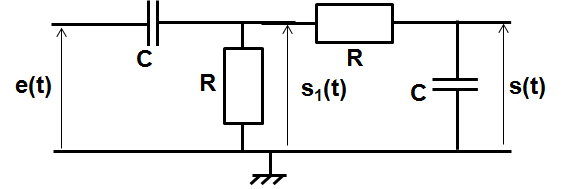
\includegraphics[scale=0.5]{images/Exo_4_3.png} 
	\end{figure}
	
	
	1. Déterminez l'expression de l'impédance formée par le circuit en aval du premier condensateur.\\
	
	2. En déduire la relation entre les tensions $e$ et $s_1$. En déduire la fonction de transfert du circuit.\\
	
	3. Quels sont les pôles et les zéros du filtre. \\
	
	4. Pour les valeurs de R et de C, tracez le diagramme asymptotique de Bode. Précisez les fréquences de coupure du filtre, ainsi que la nature du filtre.\\

	\textbf{\underline{Correction exercice 3}}\\
	
	1. Soit $Z_{eq}$ l'impédance formée par les deux résistances et le condensateur C de sortie :
	\begin{equation*}
	Z_{eq}=\frac{R(R+\frac{1}{jc\omega})}{2R+\frac{1}{jc\omega}}=\frac{R(1+jRC\omega)}{1+j2RC\omega}
	\end{equation*}	
	
	2. \begin{equation*}
	\frac{s_1}{e}=\frac{Z_{eq}}{Z_{eq}+R}=\frac{jRC\omega(1+jRC\omega)}{1+j3RC\omega-(RC)^2\omega^2}
	\end{equation*}
	On en déduit :
	\begin{equation*}
	\frac{s}{e}=\frac{s}{s_1}\frac{s_1}{e}=\frac{1}{1+jRC\omega}\frac{s_1}{e}
	\end{equation*}
	\begin{equation*}
	\frac{s}{e}=\frac{jRC\omega}{1+j3RC\omega-(RC)^2\omega^2}=\frac{1}{RC}\frac{j\omega}{1+j3RC\omega-(RC)^2\omega^2}
	\end{equation*}
	
	3. Le numérateur a une racine nulle, donc un seul zéro en f = 0. Pour les pôles, il faut déterminer les pôles du dénominateur. On trouve : $\omega_{1} = -\frac{-3+\sqrt{5}}{2RC}=\frac{0.382}{RC}$ et $\omega_{2} = -\frac{-3-\sqrt{5}}{2RC}=\frac{2.62}{RC}$\\
	
	4. Avec les valeurs de R et de C précisées, on obtient : $\omega_{1} = 3820~rad/s$ et $\omega_{2} = 26200~rad/s$. Exprimé en fréquence, cela donne : $f_1 = 608 Hz$ et $f_2=4169 Hz$. Le filtre est de type passe-bande. Il s'agit de la mise en cascade d'un filtre passe-haut et d'un filtre passe-bas.
	
	\begin{figure}[h!]
		\centering
		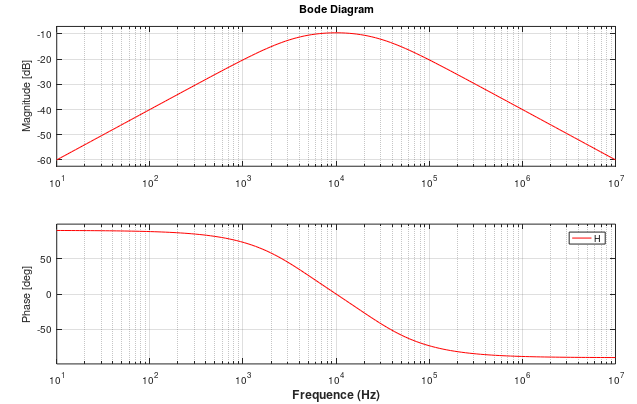
\includegraphics[scale=0.7]{images/Exo_4_3_Bode.png} 
	\end{figure}

	
	\subsubsection{Exercice 4}
	On dispose d'un filtre dont la fonction de transfert est donnée par $H(p)=\frac{1}{(p+2)^2}$.
	
	1. Tracez la réponse fréquentielle du filtre dans le diagramme de Bode. Quelle est la nature du filtre ? Quelle est sa fréquence de coupure ? \\
	
	2. Calculez sa réponse impulsionnelle.\\
	
	3. Calculez sa réponse indicielle. \\
	
	\textbf{\underline{Correction exercice 4}}\\
	
	1. Filtre passe bas d'ordre 2. La pulsation de coupure est égale à 2 rad/s, d'où une fréquence de coupure de 0.32 Hz.\\
	
	2. $h(t)=\mathcal{L}^{-1}(H(p))=\mathcal{L}^{-1}(\frac{1}{(p+2)^2})=\frac{1}{2}(1-e^{-2t})$\\
	
	3. La réponse indicielle a(t) est donnée par : $\mathcal{L}^{-1}(\frac{1}{p(p+2)^2})$, ou par l'intégration de la réponse impulsionnelle. On trouve : 
	\begin{equation*}
	a(t)=\int_{0}^{t}\frac{1}{2}(1-e^{-2\tau})d\tau = \frac{1}{4}(1-(1-2t)e^{-2t})u(t)
	\end{equation*}
	
	
	

	
	
	\subsubsection{Exercice 5 - Mise en cascade de filtres}
	On considère le filtre RC ci-dessous.
	
	\begin{figure}[h!]
		\centering
		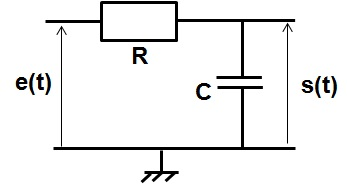
\includegraphics[scale=0.5]{images/Filtre_RC_passe_bas.jpg} 
	\end{figure}

	1. Calculez la fonction de transfert de ce filtre H(f).
	
	2. Précisez sa nature, sa fréquence de coupure, son ordre.
	
	3. On cascade deux filtres de ce type. Calculez sa fonction de transfert $H_{2}(f)$.
	
	4. Vérifie t-on $H_{2}(f)=H(f)^{2}$ ? Pourquoi ?
	
	\vspace{1\baselineskip}
	
	\textbf{\underline{Correction exercice 5}}\\
	1. $H(f)=\frac{1}{RC}\frac{1}{j2\pi f+\frac{1}{RC}}$
	
	2. Filtre passe-bas d'ordre 1. La fréquence de coupure $f_{c}=\frac{1}{2^pi RC}$
	
	3. On peut montrer que :
	\begin{equation*}
	\frac{s_{1}}{e}(p)=\frac{Z_{eq}}{R+Z_{eq}}~avec~Z_{eq}=\frac{1+RCp}{Cp(2+RCp)}
	\end{equation*}
	\begin{equation*}
	\frac{s_{1}}{e}(p)=\frac{1}{RC}\frac{p+\frac{1}{RC}}{p^{2}+\frac{3}{RC}p+\frac{1}{RC}^{2}}
	\end{equation*}
	
	\begin{figure}[h!]
		\centering
		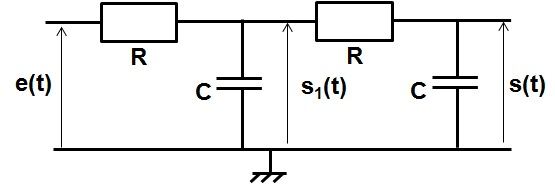
\includegraphics[scale=0.5]{images/Cascade_filtre_RC_passe_bas.jpg} 
	\end{figure}

	\begin{equation*}
	\frac{s}{s_{1}}(p)=\frac{1}{RC}\frac{1}{p+\frac{1}{RC}}
	\end{equation*}
	On en déduit l'expression de la fonction de transfert :
	\begin{equation*}
	H_{2}(p)=\frac{s}{s_{1}}(p)\cdot \frac{s_{1}}{e}(p)=\frac{1}{RC}^{2}\frac{1}{p^{2}+\frac{3}{RC}p+\frac{1}{RC}^{2}}
	\end{equation*} 
	\begin{equation*}
	\frac{s_{1}}{e}(p)=\frac{1}{RC}^{2}\frac{1}{(j2\pi f)^{2}+\frac{3}{RC}(j2\pi f)+\frac{1}{RC}^{2}}
	\end{equation*}
	On reconnait la fonction de transfert d'un filtre passe bas d'ordre 2.
	
	4. En appliquant la formule de mise en cascade des fonctions de transfert des deux cellules RC, on trouve :
	\begin{equation*}
	H(f)H(f)==\frac{1}{RC}^{2}\frac{1}{(j2\pi f)^{2}+\frac{1}{RC}(j2\pi f)+\frac{1}{RC}^{2}} \neq H_{2}(f)
	\end{equation*}
	La mise en cascade des fonctions de transfert suppose que la deuxième cellule n'influe pas sur la tension en sortie de la première cellule ($s_{1}$), ce qui n'est pas le cas. La tension mesurée $s_{1}$ dépend de l'impédance connectée en ce nœud (impédance $Z_{eq}$). La figure ci-dessous compare les fonctions de transfert $H_{2}(f)$ et $H(f)H(f)$
	
	\begin{figure}[h!]
		\centering
		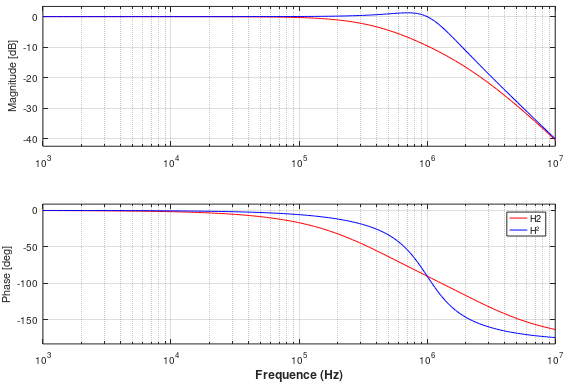
\includegraphics[scale=0.6]{images/Effet_cascade_filtre_RC.png} 
	\end{figure}
	
	 
	
	
	
	
	
	
	
	\vspace{1\baselineskip}
	
	
	\newpage
	
	\chapter{Séries de Fourier - Analyse fréquentielle des signaux périodiques}
	
	\subsubsection{Exercice 1}
	Développez en série de Fourier la fonction $f(t)=|sin(\alpha t)|$ avec $\alpha \in \mathbb{R^{*}}$ donné.\\
	
	\subsubsection{Exercice 2}
	Soit f : $\mathbb{R} \rightarrow \mathbb{R}$ une fonction périodique de période 4, impaire, définie par :
	\begin{equation*}
	f(t)=\left \{
	\begin{array}{l}
	1-t~~si~t~\in[0;1[ \\
	0~~si~t~\in[1;2[ \\
	\end{array}
	\right .
	\end{equation*}
	
	1. Dessinez le graphe de f. Calculer f(7), f($\frac{9}{2})$ et $f(\frac{11}{2})$.\\
	
	2. Calculez les coefficients de Fourier de f.\\
	
	\subsubsection{Exercice 3}
	Cet exercice est en relation avec l'exemple d'un signal rectangulaire présenté dans le cours. On considère un signal de même nature, de moyenne nulle, de période $T_1$, de fréquence $f_1$ et	d'amplitude 2, représenté par la fonction périodique s. On s'intéresse au produit scalaire de la fonction s avec les fonctions de base $cos(n\omega_{1}t)$, n = 1, 2 et 3 où $\omega_{1} = \frac{2\pi}{T_1}$. La figure ci-dessous représente sur la première ligne, dans la colonne de gauche, le graphe de la fonction s superposé à celui de	la fonction $cos(\omega_{1}t)$ et dans la colonne de droite, le graphe du produit scalaire $s(t)cos(\omega_{1}t)$ sur
	une période $T_1$. Sur la deuxième ligne sont représentés, dans la colonne de gauche, le graphe de la fonction s superposé à celui de la fonction $cos(2\omega_{1}t)$ et dans la colonne de droite, le graphe	du produit scalaire $s(t)cos(2\omega_{1}t)$ sur une période $T_1$. Sur la troisième ligne sont représentés,
	dans la colonne de gauche, le graphe de la fonction s superposé à celui de la fonction  $cos(3\omega_{1}t)$	et dans la colonne de droite, le graphe du produit scalaire $s(t)cos(3\omega_{1}t)$ sur une période $T_1$. 
	
	\begin{figure}[h!]
		\centering
		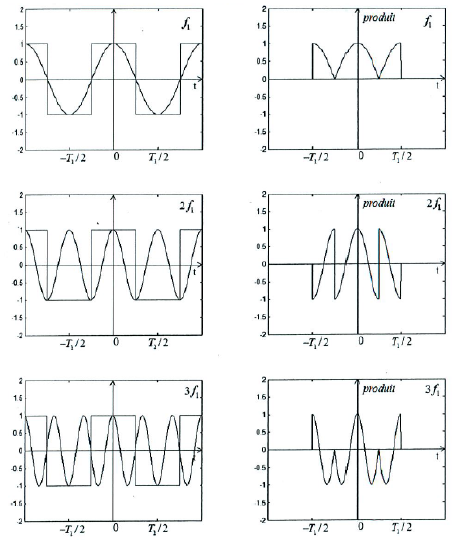
\includegraphics[scale=0.8]{images/Exo_Fourier_Lea.png}
		\caption{Colonne de gauche : graphe de s et de $cos(\omega_{1}t)$, $cos(2\omega_{1}t)$, $cos(3\omega_{1}t)$ - Colonne de droite
			: graphes de $s(t)cos(\omega_{1}t)$, $s(t)cos(2\omega_{1}t)$ et $s(t)cos(3\omega_{1}t)$.}	
		\label{Fig:Exo_Fourier_signal_carré} 
	\end{figure}
	
	1. Définir la fonction s.\\
	2. Que représente le produit scalaire de s par une fonction de base $cos(n\omega_{1}t)$, n = 1, 2 ou 3 ?\\
	3. Interpréter qualitativement (sans calcul) les trois produits scalaires représentés sur la figure \ref{Fig:Exo_Fourier_signal_carré} en donnant leur signe et une indication de leur valeur algébrique.\\
	4. A quel résultat (sans calcul) peut-on s'attendre si on effectue le produit scalaire de s par les fonctions de bases $sin(n\omega_{1}t)$, n = 1, 2 ou 3 ? ?\\
	5. En considérant le signal s comme un signal retardé par rapport au signal étudié en
	cours et en utilisant les résultats établis dans le cours, calculer les coefficients de Fourier exponentiels de s. Donner la série de Fourier associée à s.\\
	
	
	\subsubsection{Exercice 4}
	Soit f une fonction définie sur l'intervalle [0;1] de $\mathbb{R}$ par f(t) = t.
	On considère f comme la restriction de fonctions $g_i$ avec i = 1, 23 3, périodiques et continues par morceaux sur $\mathbb{R}$. On se propose de déterminer plusieurs expressions de f sur ]0;1[ à partir du développement en séries de Fourier des fonctions $g_i$.\\
	
	1. On considère la fonction $g_1$, périodique, de période $T_1$ = 3, définie par $\forall t \in [0;3[~~ g_1(t) = t$.\\
	a. Représentez la fonction $g_1$ sur l'intervalle [-3;6].
	
	b. Calculez les coefficients de Fourier de $g_1$ et donnes la série de Fourier $S_1$ associée à $g_1$.
	
	
	c. Etudiez la convergence de $S_1$.
	
	d. En déduire le développement en série de Fourier de f sur ]0;1[.\\
	
	2. On considère la fonction $g_2$, impaire, périodique, de période $T_2$ = 2, définie par $\forall t \in [0;1[~~ g_2(t) = t$.\\
	a. Représentez la fonction $g_2$ sur l'intervalle [-3;3].
	
	b. Calculez les coefficients de Fourier de $g_2$ et donnes la série de Fourier $S_2$ associée à $g_2$.
	
	c. Etudiez la convergence de $S_2$.
	
	d. En déduire le développement en série de Fourier de f sur ]0;1[.\\
	
	3. On considère la fonction $g_3$, paire, périodique, de période $T_3$ = 2, définie par $\forall t \in [0;1[~~ g_3(t) = t$.\\
	a. Représentez la fonction $g_3$ sur l'intervalle [-4;4].
	
	b. Calculez les coefficients de Fourier de $g_3$ et donnes la série de Fourier $S_3$ associée à $g_3$.
	
	c. Etudiez la convergence de $S_3$.
	
	d. En déduire le développement en série de Fourier de f sur ]0;1[.\\
	
	
	\subsubsection{Exercice 5}
	
	Donnez la définition, la période et la parité des fonctions représentées par les séries de Fourier suivantes et tracez leur graphe :\\
	
	1. $	\frac{2}{\pi}-\frac{4}{\pi}\sum_{n=1}^{+\infty}cos(2nt)=sin(t)~~avec~t~\in[0;\pi]$\\
	
	2. $	2\sum_{n=1}^{+\infty}\frac{1-(-1)^{n}}{n \pi}sin(n \pi t)=1~~avec~t~\in[0;1]$ \\
	
	3. $	\pi-\sum_{n=1}^{+\infty}\frac{2}{n}sin(nt)=t~~avec~t~\in[0;2\pi]$ \\
	
	
	\subsubsection{Exercice 6 - Signal de forme exponentielle}
	On considère la fonction x définie sur $\mathbb{R}$ à valeurs dans $\mathbb{R}$, de période $T=2\pi$, par $x(t)=e^{t}$ pour $t\in [0;+2\pi[$.\\
	
	1. Tracez la fonction x(t) sur l'intervalle $[-2\pi;+2\pi[$.\\
	
	2. Cette fonction admet-elle un développement en série de Fourier ?\\
	
	3. Montrez que les coefficients de Fourier sous la forme exponentielle sont égaux à $c_{n}=\frac{1+jn}{2\pi(1+n^{2})}(e^{2\pi}-1)~~\forall n \in \mathbb{Z}$.\\
	
	4. En déduire les expressions des coefficients de Fourier sous leur forme trigonométriqque.\\
	
	5. Calculez la puissance moyenne des harmoniques, quelle que soit leur rang.\\
	
	6. Calculez la puissance moyenne du signal.\\
	
	
	
	
	\subsubsection{Exercice 7 - Modulation à largeur d'impulsion}
	La modulation à largeur d'impulsion (MLI) (Pulse Width Modulation PWM en anglais) est une technique couramment utilisée en électronique pour générer un signal analogique à partir d'un signal discret à deux états. Le signal MLI $s_p(t)$ est constitué d'une suite périodique, de période T, d'impulsions $s_i(t)$ définie par :
	\begin{equation*}
	s_i(t)=\left \{
	\begin{array}{l}
	A~~si~t~\in[0;\alpha T] \\
	0~~sinon \\
	\end{array}
	\right .
	\end{equation*}   
	où $\alpha \in [0;1]$ est appelé le rapport cyclique du signal (duty ratio en anglais). Le principe est illustré à la figure \ref{Fig:signal_MLI}. A partir d'un signal analogique de valeurs comprises entre 0 et A, un modulateur MLI va produire le signal MLI à partir de deux niveaux de tension seulement.\\
	
	\begin{figure}[h!]
		\centering
		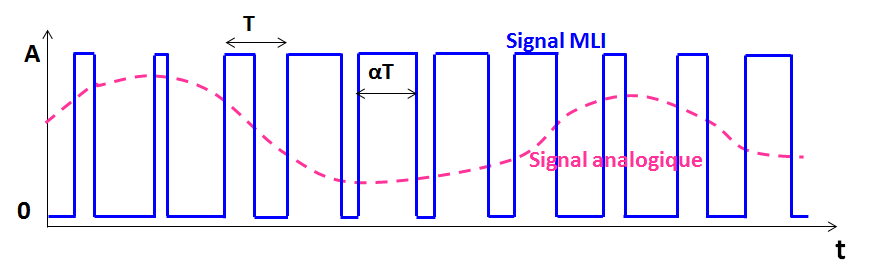
\includegraphics[scale=0.6]{images/signal_MLI.png}
		\caption{Illustration modulation MLI}	
		\label{Fig:signal_MLI} 
	\end{figure}
	
	1. Vérifiez si on peut développer $s_i(t)$ et $s_p(t)$ en séries de Fourier. \\
	
	2. Calculez les coefficients de Fourier exponentiels du signal MLI $s_p(t)$ et vérifiez la relation avec les coefficients de Fourier réels.\\
	
	3. Que deviennent ces coefficients si l'on considère le signal $s_p(t)$ de même période mais retardé d'un temps $\tau \in \mathbb{R^{*}}$.\\
	
	4. Calculez la puissance moyenne du signal, ainsi que celles de la somme de tous les termes de la série de Fourier. Sont-elles égales ?\\
	
	5. Quelle est la puissance moyenne transportée par le premier harmonique ?\\
	
	6. Une manière économique de reconstituer un signal analogique à partir du signal MLI est de le filtrer, à l'aide d'un filtre passe-bas que l'on supposera idéal. Sa fréquence de coupure est notée $f_c$. Quelle est la forme du signal selon $f_c$ ? Quelle fréquence de coupure choisiriez-vous pour que le signal en sortie du filtre soit constant et proportionnel au rapport cyclique ? Est-ce un bon choix pour reconstituer le signal analogique ?\\
	
	7. Quelle est l'énergie du signal en sortie du filtre ? En déduire le rendement du système de conversion ?\\
	
	\newpage
	
	
	\chapter{Transformée de Fourier}
	
	\subsubsection{Exercice 1}
	
	On considère le signal $s_1$ défini pour tout réel t par :
	\begin{equation*}
	s_1(t)=e^{-at}u(t)
	\end{equation*}
	où u(t) est la fonction échelon de Heaviside et $a \in \mathbb{R_{+}^{*}}$. Tracez le graphe de $s_1$. Déterminez sa transformée de Fourier $S_1$.\\
	
	2. En utilisant les propriétés de la transformée de Fourier, déterminer après avoir tracé le graphe des signaux $s_2$ et $s_3$ :
	
	a. la transformée de Fourier $S_2$ du signal $s_2$ défini pour tout réel t par $s_2(t)=e^{at}u(-t)$.\\
	
	b.la transformée de Fourier $S_3$ du signal $s_3$ défini pour tout réel t par $s_2(t)=e^{-a|t|}$.\\
	
	c. la transformée de Fourier $S_4$ du signal $s_4$ défini pour tout réel t par $s_4(t)=-e^{at}u(-t)+e^{-at}u(t)$.\\
	
	\subsubsection{Exercice 2}
	
	Calculez les transformées de Fourier de signaux suivants :\\
	
	a. $v(t) = cos(2\pi f_0 t)\pi_{T_0}(t)$\\
	
	b. $w(t) = \delta(t-T_e)+\delta(t)+\delta(t+T_e)$\\
	
	c. $x(t) = \delta(t-2T_e)+\delta(t)+\delta(t+2T_e)$\\
	
	d. $x(t) = te^{-at}u(t)~,~~a>0$\\
	
	e. La fonction y(t) décrite sur la figure \ref{Fig:Exo_TF_2}.
	
	\begin{figure}[h!]
		\centering
		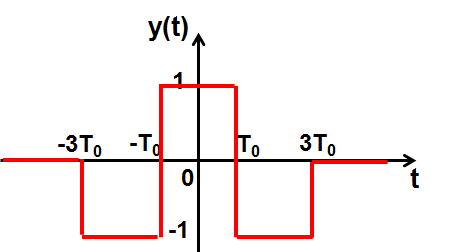
\includegraphics[scale=0.5]{images/exo_2_TF.png}
		\caption{Figure exercice 2}	
		\label{Fig:Exo_TF_2} 
	\end{figure}
	
	
	\subsubsection{Exercice 3 - Signal numérique}
	On considère l'impulsion de forme trapézoïdale présentée sur la figure \ref{Fig:Exo_TF_3}. Celle-ci constitue un modèle simplifié des signaux électriques numériques.\\
	
	\begin{figure}[h!]
		\centering
		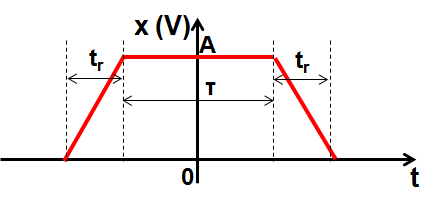
\includegraphics[scale=0.6]{images/exo_3_TF.png}
		\caption{Figure exercice 3}	
		\label{Fig:Exo_TF_3} 
	\end{figure}
	
	1. Calculez la transformée de Fourier du signal.\\
	
	2. Esquissez l'allure de son spectre (module seulement). Précisez l'unité.\\
	
	3. Calculez l'énergie de ce signal.\\
	
	4. Le spectre est-il à bande limitée ? Quelle(s) paramètre(s) affectent l'occupation spectrale du signal ?\\
	
	
	
	\subsubsection{Exercice 4}
	Soit un filtre passe-bas RC, avec R = 1 k$\Omega$ et C = 1 $\mu$F. On envoie en entrée un signal $x(t)=e^{-10^{3}t}u(t)$.\\
	
	1. Etablir la fonction de transfert du filtre en fonction de la fréquence.\\
	
	2. Calculez la transformée de Fourier X(f) du signal x(t).\\
	
	3. Déterminez le spectre de la réponse du filtre.\\
	
	4. Calculez la réponse du filtre dans le domaine temporel.\\
	
	
	
	\newpage
	
	\chapter{Analyse des systèmes et des signaux dans le domaine temporel}
	
	\subsubsection{Exercice 1}
	
	Déduire les réponses impulsionnelles des systèmes décrits par les fonctions ci-dessous :\\
	a. $G(p)=\frac{1}{p(p+2)}+\frac{1}{2}(\frac{e^{4}}{p+2}-\frac{1}{p})e^{-2p}$ \\
	b. $H(j\omega)=\frac{2j\omega}{2+j\omega}$\\
	c. $a(t)=t^{2}u(t)$ où a(t) est la réponse indicielle \\
	d. $a(t)=u(t)(2-e^{-t})$ où a(t) est la réponse indicielle
	
	
	\textbf{\underline{Correction exercice 1}}\\
	
	a. $G(p)=\frac{1}{2p}-\frac{1}{2(p+2)}+\frac{1}{2}(\frac{e^{4}}{p+2}-\frac{1}{p})e^{-2p}$ \\
	$g(t)=\mathcal{L}^{-1}[H(p)]=\frac{1}{2}(1-e^{-2t})u(t)+\frac{1}{2}(e^{4}e^{-2t}-1)u(t-2)$\\
	
	b.Par transformée de Fourier inverse, on peut identifier  : $h(t)=2\frac{d}{dt}(e^{-2t}u(t))=-4e^{-2t}u(t)+2\delta(t)$. On peut aussi remarquer que : $H(p)=2(1-\frac{2}{2+j\omega})$. On identifie facilement la transformée de Fourier inverse : $2\delta(t)-4e^{-2t}u(t)$.\\
	
	c. $h(t)=\frac{da(t)}{dt}=2tu(t)+t^{2}\delta(t)=2tu(t)$\\
	
	d. $h(t)=\frac{da(t)}{dt}=\delta(t)(2-e^{-t})+e^{-t}u(t)=2\delta(t)+e^{-t}u(t)$
	
	\vspace{1\baselineskip}
	
	\subsubsection{Exercice 2}
	
	Calculez les produits de convolution suivants : \\
	a. $e(t)=u*u(t)$ avec $t \in \mathbb{R}$\\
	b. $f(t)=sin(t)*\Pi_{2a}(t)$ avec $t \in \mathbb{R}$\\
	c. $g(t)=cos(t)*\Pi_{2a}(t)$ avec $t \in \mathbb{R}$\\
	d. $h(t)=\Pi_{2a}(t)*e^{-bt}$ avec $t \in \mathbb{R}$\\
	e. $m(t)=(\delta(t-1)-\delta(t-2))*(u(t+1)-u(t-1))$ avec $t \in \mathbb{R}$
	
	\vspace{1\baselineskip}
	
	\textbf{\underline{Correction exercice 2}}\\
	
	a. $e(t)=\int_{-\infty}^{t}u(\tau)d\tau=\int_{0}^{t}d\tau=t\cdot u(t)$\\
	b. $f(t)=\int_{t-a}^{t+a}sin(\tau)d\tau=[-cos(\tau)]_{t-a}^{t+a}=f(t)=2sin(t)sin(a)$\\
	c. $g(t)=\int_{t-a}^{t+a}cos(\tau)d\tau=[sin(\tau)]_{t-a}^{t+a}=f(t)=2cos(t)sin(a)$\\
	d. $h(t)=\int_{t-2a}^{t}e^{-b\tau}d\tau=-\frac{1}{b}[e^{-b\tau}]_{t-2a}^{t}=\frac{e^{bt}}{b}(e^{2ab}-1)$\\
	e. On pose : $n(t)=\delta(t-1)-\delta(t-2)$ et $p(t)=u(t+1)-u(t-1)$. Etant donnée la propriété d'échantillonnage de l'impulsion de Dirac :
	\begin{equation*}
	m(t)=n*p(t)=p(t-1)-p(t-2)=(u(t)-u(t-2))-(u(t-1)-u(t-3))
	\end{equation*}
	Autrement dit : m(t) = 1 si $0 \leq t < 1$, m(t) = -1 si $2 \leq t < 3$, m(t)=0 sinon. 
	
	
	\vspace{1\baselineskip}
		
	\subsubsection{Exercice 3}
	
	On considère les fonctions h(t) et x(t) dont le profil est représenté ci-dessous.
	\begin{figure}[h!]
		\centering
		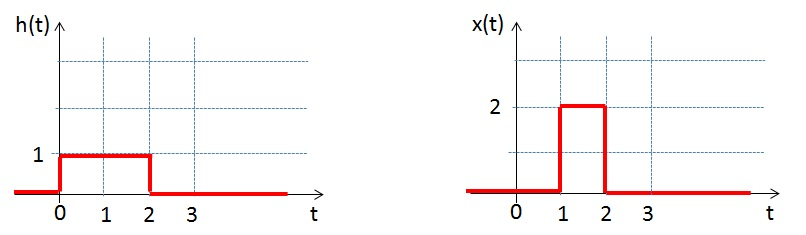
\includegraphics[scale=0.5]{images/Courbes_TD_Convolution_2.jpg} 
	\end{figure}
	
	1. Proposez une expression mathématique pour ces deux fonctions.
	
	2. On note y(t) le résultat du produit de convolution de x(t) et h(t). Déterminez l'expression de y(t) en calculant directement le produit de convolution. Tracez l'allure de cette fonction.
	
	3. En utilisant la transformée de Laplace, vérifiez la validité du résultat précédent.
	
	4. Même chose en utilisant la transformée de Fourier.
	
	\vspace{1\baselineskip}
	
	\textbf{\underline{Correction exercice 3}}\\
	
	1. $h(t)=u(t)-u(t-2)$ et $x(t)=2(u(t-1)-u(t-2))$.
	
	2. Graphiquement, on peut déduire l'allure de $y(t)=\int_{-\infty}^{+\infty}h(\tau)x(t-\tau)d\tau$. En traçant $h(\tau)$ et $x(t-\tau)$, on distingue 5 intervalles différents :
	\begin{itemize}
		\item si t < 1 ou t > 4, alors $h(\tau)$ et $x(t-\tau)$ ne se recouvrent jamais, donc l'intégrale $y(t)=\int_{-\infty}^{+\infty}h(\tau)x(t-\tau)d\tau = 0$.
		\item si $1 \leq t<2$, alors l'aire sous l'intersection des courbes $h(\tau)$ et $x(t-\tau)$ croit linéairement quand t augmente.
		\item si $2 \leq t < 3$, alors l'aire sous l'intersection des courbes $h(\tau)$ et $x(t-\tau)$ est maximale, constante et égale à 2.
		\item si $3 \leq t < 4$,  alors l'aire sous l'intersection des courbes $h(\tau)$ et $x(t-\tau)$ décroit linéairement quand t augmente.
	\end{itemize}
	
	L'allure de y(t) est présentée ci-dessous. On peut en déduire l'expression suivante :
	\begin{equation*}
	y(t)=2[(t-1)u(t-1)-(t-2)u(t-2)-(t-3)u(t-3)+(t-4)u(t-4)]
	\end{equation*}
	\begin{figure}[h!]
		\centering
		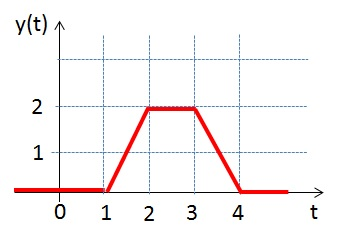
\includegraphics[scale=0.6]{images/Courbes_TD_Convolution_2_Solution.jpg} 
	\end{figure}

	Cette expression peut aussi être déduite en résolvant directement l'intégrale du produit de convolution :
	\begin{equation*}
	y(t)=2\int_{-\infty}^{+\infty}(u(\tau)-u(\tau-2))\cdot (u(t-(\tau-1))-u(t-(\tau-2)))d\tau
	\end{equation*}
	\begin{equation*}
	y(t)=2\int_{-\infty}^{+\infty}[u(\tau)u(t-(\tau-1))-u(\tau)u(t-(\tau-2))-u(\tau-2)u(t-(\tau-1))+u(\tau-2)u(t-(\tau-2))]d\tau
	\end{equation*}
	On distingue quatre termes dans l'intégrale, qui peuvent être calculés individuellement :
	\begin{itemize}
		\item $\int_{-\infty}^{+\infty}u(\tau)u(t-(\tau-1))d\tau=(t-1)u(t-1)$
		\item $\int_{-\infty}^{+\infty}u(\tau)u(t-(\tau-2))d\tau=(t-2)u(t-2)$
		\item $\int_{-\infty}^{+\infty}u(\tau-2)u(t-(\tau-1))d\tau=(t-3)u(t-3)$
		\item $\int_{-\infty}^{+\infty}u(\tau-2)u(t-(\tau-2))d\tau=(t-4)u(t-4)$
	\end{itemize}
	En addition ces différentes contributions, on retrouve le résultat précédent :
	$y(t)=2[(t-1)u(t-1)-(t-2)u(t-2)-(t-3)u(t-3)+(t-4)u(t-4)]$.
	
	\vspace{0.5\baselineskip}
	
	3. La validité du résultat précédent peut facilement être vérifiée en utilisant la transformée de Laplace. En effet, le produit de convolution se transforme en un simple produit dans le domaine des fréquences complexes.
	Les transformées de Laplace de h(t) et x(t) peuvent facilement être dérivées à partir de la table des transformées de Laplace courantes : $H(p) = \frac{1}{p}-\frac{e^{-2p}}{p}$ et $X(p)=\frac{2e^{-p}}{p}-\frac{2e^{-2p}}{p}$. La transformée de Laplace Y(p) est déterminée en multipliant les deux termes précédents :
	\begin{equation*}
	Y(p)=(\frac{1}{p}-\frac{e^{-2p}}{p})\cdot(\frac{2e^{-p}}{p}-\frac{2e^{-2p}}{p})=\frac{2e^{-p}}{p^{2}}-\frac{2e^{-2p}}{p^{2}}-\frac{2e^{-3p}}{p^{2}}+\frac{2e^{-4p}}{p^{2}}
	\end{equation*}
	En utilisant la transformée de Laplace inverse, on retrouve la même expression pour y(t) que dans la question précédente.
	
		$y(t)=\mathcal{L}^{-1}[Y(p)]=2[(t-1)u(t-1)-(t-2)u(t-2)-(t-3)u(t-3)+(t-4)u(t-4)]$
	
	\vspace{0.5\baselineskip}
	
	4. Le même genre de vérification peut être réalisée en utilisant la transformée de Fourier. Les fonctions h(t) et x(t) sont deux fonctions portes de largeur T=2 et T=1 respectivement. Elles sont centrées sur 1 et 1.5 respectivement. Leurs transformées de Fourier sont données par :
	\begin{equation*}
	H(f)=2sinc(2f)e^{j2\pi f}=2\frac{sin(2\pi f)}{2\pi f}e^{j2\pi f}
	\end{equation*}
	\begin{equation*}
	X(f)=2sinc(f)e^{j2\pi f\cdot \frac{3}{2}}=2\frac{sin(\pi f)}{\pi f}e^{j2\pi f\cdot \frac{3}{2}}
	\end{equation*}
	La transformée de Fourier de y(t) est obtenue en multipliant les deux termes précédents.
	\begin{equation*}
	Y(f)=H(f) \cdot X(f) = 4sinc(2f)sinc(f)e^{j2\pi f\cdot \frac{5}{2}}
	\end{equation*}
	Cette expression peut être simplifiée en développant le terme $sinc(2f)$ pour faire apparaître deux termes $sinc(f)$ :
	\begin{equation*}
		Y(f)=4\frac{sin(2\pi f)}{2\pi f}sinc(f)e^{j2\pi f\cdot \frac{5}{2}}
	\end{equation*}
	\begin{equation*}
	Y(f)=4\frac{2sin(\pi f)cos(\pi f)}{2\pi f}sinc(f)e^{j2\pi f\cdot \frac{5}{2}}
	\end{equation*}
	\begin{equation*}
	Y(f)=4\frac{sin(\pi f)}{\pi f}\frac{e^{j\pi f}+e^{-j\pi f}}{2}sinc(f)e^{j2\pi f\cdot \frac{5}{2}}
	\end{equation*}
	\begin{equation*}
	Y(f)=2(sinc(f))^{2}(e^{j2\pi f\cdot 3}+e^{-j2\pi f\cdot 2})=2(a(t)+b(t))
	\end{equation*}
	
	Dans l'expression ci-dessous, on trouve le terme $(sinc)^{2}$, qui correspond à une fonction rectangulaire. Le terme suivant, entre parenthèses, indique la somme de deux fonctions triangulaires décalées dans le temps : la première (a(t)) est centrée sur t=3, la seconde (b(t)) sur t=2. C'est ce qu'illustre la figure ci-dessous.
	\begin{figure}[h!]
		\centering
		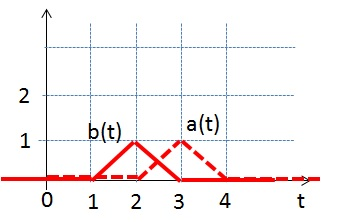
\includegraphics[scale=0.6]{images/Courbes_TD_Convolution_2_Solution_2.jpg} 
	\end{figure}
	En écrivant $a(t)=(t-2)(u(t-3)-u(t-2))+(4-t)(u(t-3)-u(t-4))$ et $b(t)=(t-1)(u(t-1)-u(t-2))+(3-t)(u(t-2)-u(t-3))$, on retrouve l'expression précédente pour y(t).
	
	\vspace{1\baselineskip}
	
	\subsubsection{Exercice 4}
	On considère un filtre linéaire à temps invariant dont la fonction de transfert est donnée par $H(\omega)=\frac{j\omega}{1+j\omega}$. 
	
	1. On l'excite à l'aide d'un signal échelon. Calculez la réponse du filtre en utilisant sa réponse impulsionnelle. Esquissez sa forme temporelle.\\
	
	2. Même question si on excite le filtre à partir du signal $e(t)=u(t)-u(t-2)$. 
	
	\vspace{1\baselineskip}
	
	\textbf{\underline{Correction exercice 4}}\
	
	1. On établit d'abord la réponse impulsionnelle du filtre (passe-haut) : $h(t)=-e^{-t}u(t)+\delta(t)$. L'excitation du filtre est : $e(t)=u(t)$.
	La réponse y(t) du filtre est donnée par :
	
	\begin{equation*}
	y(t)=h*x(t)=\int_{-\infty}^{+\infty}(-e^{-\tau}u(\tau)+\delta(\tau))u(t-\tau)d\tau
	\end{equation*}
	\begin{equation*}
	y(t)=\int_{-\infty}^{+\infty}-e^{-\tau}u(\tau)u(t-\tau)d\tau+\int_{-\infty}^{+\infty}\delta(\tau)u(t-\tau)d\tau
	\end{equation*}
	\begin{equation*}
	y(t)=\int_{0}^{t}-e^{-\tau}d\tau+1=e^{-t}~~si~t\geq 0
	\end{equation*}
	\begin{equation*}
	y(t)=0~~sinon
	\end{equation*}
	
	2. $y(t)=h*e(t)=h*u(t)-h*u(t-2)$
	
	On montre que $h*u(t-2)=(1-e^{-2}+e^{-t})u(t-2)$. On en déduit :
	\begin{equation*}
	y(t)=e^{-t}u(t)-(1-e^{-2}+e^{-t})u(t-2)
	\end{equation*}
	
	\vspace{1\baselineskip}
	
	\subsubsection{Exercice 5 - Convolution de spectre}
	
	On considère deux signaux, définis par les fonctions $f_{1}(t) = cos(\omega_{1}t) et f_{2} = cos(\omega_{2}t)$. 
	
	1. Déterminez l'expression du spectre du signal $f(t)=f_{1}(t)\cdot f_{2}(t)$ (on prendra $\omega_{1} > \omega_{2}$). Représentez le graphiquement.
	
	2. Même chose avec $f_{2}(t) = sin(\omega_{2}t)$.
	
	3. Même chose avec $f_{2}(t) = sinc(t)$.
	
	4. Conclure sur l'effet de la multiplication par un signal sinusoïdal.
	
	\vspace{1\baselineskip}
	
	\textbf{\underline{Correction exercice 5}}\\
	
	1. On détermine d'abord les spectres des signaux $f_{1}$ et $f_{2}$ : $F_{1}(\omega)=\frac{\delta(\omega-\omega_{1})+\delta(\omega+\omega_{1})}{2}$ et $F_{2}(\omega)=\frac{\delta(\omega-\omega_{2})+\delta(\omega+\omega_{2})}{2}$.
	La multiplication de deux signaux dans le domaine temporel conduit à un produit de convolution de leur spectre :
	
	\begin{equation*}
	F(\omega)=F_{1}*F_{2}(\omega)=\frac{1}{4}[(\delta(\omega-\omega_{1})+\delta(\omega+\omega_{1}))*(\delta(\omega-\omega_{2})+\delta(\omega+\omega_{2})]
	\end{equation*}
	\begin{equation*}
	F(\omega)=\frac{1}{4}[\delta(\omega-\omega_{1})*\delta(\omega-\omega_{2})+\delta(\omega-\omega_{1})*\delta(\omega+\omega_{2})+\delta(\omega+\omega_{1})*\delta(\omega-\omega_{2})+\delta(\omega+\omega_{1})*\delta(\omega+\omega_{2})]
	\end{equation*}
	\begin{equation*}
	F(\omega)=\frac{1}{4}[\delta(\omega-(\omega_{1}+\omega_{2}))+\delta(\omega-(\omega_{1}-\omega_{2}))+\delta(\omega-(-\omega_{1}+\omega_{2}))+\delta(\omega-(-\omega_{1}-\omega_{2}))]
	\end{equation*}
	Dans les fréquences positives, la multiplication de ces deux signaux a conduit à deux nouvelles composantes harmoniques, de fréquences $\omega_{1}-\omega_{2}$ et $\omega_{1}+\omega_{2}$. Tout se passe comme s'il y avait eu une translation du spectre du signal $f_{1}$ d'une fréquence = $+/-\omega_{2}$ (ou inversement du spectre du signal $f_{2}$ d'une fréquence = $+/-\omega_{1}$).
	
	2. $F_{2}(\omega)=\frac{\delta(\omega-\omega_{2})-\delta(\omega+\omega_{2})}{2j}$
	
	\begin{equation*}
	F(\omega)=F_{1}*F_{2}(\omega)=\frac{1}{4j}[\delta(\omega-(\omega_{1}+\omega_{2}))-\delta(\omega-(\omega_{1}-\omega_{2}))+\delta(\omega-(-\omega_{1}+\omega_{2}))-\delta(\omega-(-\omega_{1}-\omega_{2}))]
	\end{equation*}
	
	On retrouve le même genre de spectre qu'à la question précédente, à la phase près.
	
	3. $F_{2}(\omega)=\Pi_[-1;1](\omega)$.
	
	\begin{equation*}
		F(\omega)=F_{1}*F_{2}(\omega)=\frac{1}{2}[(\delta(\omega-\omega_{1})+\delta(\omega+\omega_{1}))*\Pi_[-1;1](\omega)]
	\end{equation*}
	\begin{equation*}
	F(\omega)=\frac{1}{2}[\Pi_[-1;1](\omega-\omega_{1})+\Pi_[-1;1](\omega+\omega_{1})]
	\end{equation*}
	
	Le spectre du signal de sortie correspond de $+/-\omega_{1}$ du signal $f_{2}$.
	
	
	\vspace{1\baselineskip}
	
	
	\subsubsection{Exercice 6}
	
	On considère la fonction porte $\pi_{[-a;a]}(t)=\pi(t)$ avec $a \in \mathbb{R^{*}}$.\\
	
	1. Calculez le produit de convolution $s(t)=\pi(t)*\pi(t)$.
	
	2. Calculez la transformée de Fourier $\Pi(f)$ de la fonction $\pi(t)$. En déduire l'expression de la transformée de Fourier S(f) de la fonction s(t).
	
	3. Soit le signal $l(t)=\pi(t) \cdot \pi(t)$. Calculez la transformée de Fourier L(f) de la fonction l(t).\\
	
	On pose a = 0.5. On considère $t \in \mathbb{R}$.
	
	4. Calculez le produit de convolution $p(t)=\pi(t)*\pi(\frac{t}{2})$.
	
	5. On considère les fonctions définies par $s_{1}(t)=\pi(\frac{t-1}{2})$ et $s_{2}(t)=s_{1}(t)-s_{1}(t-2)$. Tracez $s_{1}(t)$ et $s_{2}(t)$. Calculez le produit de convolution entre $s_{1}$ et $s_{2}$.
	
	\vspace{1\baselineskip}
	
	\textbf{\underline{Correction exercice 6}}\\
	
	1. $s(t)=t+2a$ si $t \in [-2a;0]$, $s(t)=2a-t$ si $t \in [0;2a]$, s(t)=0 sinon. Il s'agit de la fonction triangle centrée sur 0, que l'on note : $2a\Delta_{2a}(t)$.\\
	
	2. Transformée de Fourier de la fonction porte : $\Pi(f)=2asinc(2\pi af)$
	On en déduit celle de la fonction s(t) : 
	\begin{equation*}
	S(f)=\Pi(f) \cdot \Pi(f) = 4a^{2}(sinc(2\pi af))^{2}
	\end{equation*}
	
	3. La première méthode consiste à utiliser l'équivalence multiplication - produit de convolution dans les domaines temporels et fréquentiels. Cependant, elle oblige à faire une convolution entre deux fonction sinc (transformée de Fourier de la fonction porte).
	La seconde approche, plus simple, consiste à se rendre compte que $\pi(t) \cdot \pi(t) = \pi(t)$. On en déduit donc la transformée de Fourier du signal l(t) :
	\begin{equation*}
	L(f)=\mathcal{F}[\pi(t)]=2asinc(2\pi af)
	\end{equation*}
	
	4. En prenant $a=\frac{1}{2}$, on a $\pi(t) = 1 si t \in [-1;1]$, et $\pi(t/2) = 1 si t \in [-2;2]$. Une manière de faire le calcul est de remarquer que :
	\begin{equation*}
	\pi(t/2) = \pi(t+\frac{1}{2})+\pi(t-\frac{1}{2})
	\end{equation*}
	Ainsi, on va faire des produits de convolution entre deux fonctions portes de même largeur, que l'on a déjà calculé à la première question :
	\begin{equation*}
	p(t)=\pi(t)*\pi(t/2)=\pi(t)*(\pi(t+\frac{1}{2})+\pi(t-\frac{1}{2}))
	\end{equation*}
	\begin{equation*}
	p(t)=\pi(t)*\pi(t+\frac{1}{2})+\pi(t)(\pi(t-\frac{1}{2})
	\end{equation*}
	L'ajout de 1/2 dans les abscisses des fonctions portes conduit à un décalage de +/-1/2.
	\begin{equation*}
	p(t)=2a\Delta_{2a}(t+\frac{1}{2})+2a\Delta_{2a}(t-\frac{1}{2})=\Delta_{1}(t+\frac{1}{2})+\Delta_{1}(t-\frac{1}{2})
	\end{equation*}
	
	5. La fonction $s_{1}(t)$ est une fonction porte de largeur 2 et centrée sur 1. La fonction $s_{1}(t-2)$ est une version décalée de $s_{1}(t)$, centrée sur 3.
	
	\begin{figure}[h!]
		\centering
		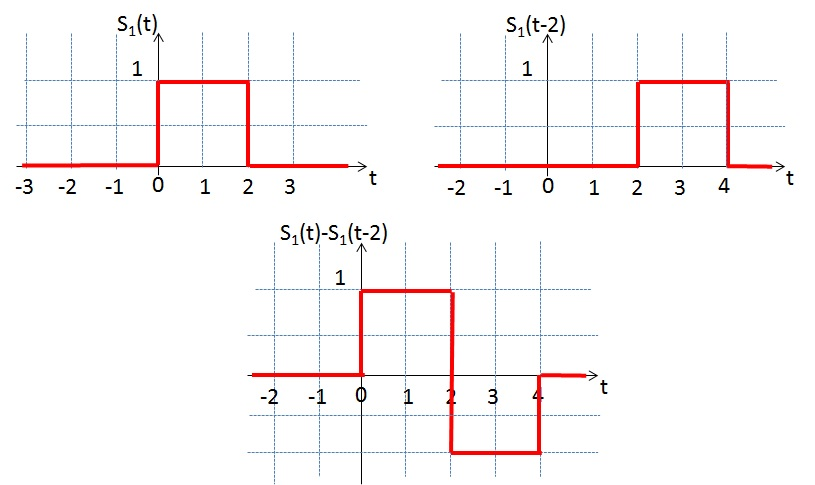
\includegraphics[scale=0.6]{images/TD_7_exo6.jpg} 
	\end{figure}

	\begin{equation*}
	s_{1}*s_{2}(t)=s_{1}*s_{1}(t)-s_{1}(t)*s_{1}(t-2)
	\end{equation*}
	Premier terme : 
	\begin{equation*}
	s_{1}*s_{1}(t)=\pi(\frac{t-1}{2})*\pi(\frac{t-1}{2})=2\Delta(\frac{t-2}{4})
	\end{equation*}
	Second terme : 
	\begin{equation*}
	s_{1}(t)*s_{1}(t-2) = \pi(\frac{t-1}{2})*\pi(\frac{t-3}{2})=2\Delta(\frac{t-4}{4})
	\end{equation*}
	D'où : $s_{1}*s_{2}(t)=2\Delta(\frac{t-2}{4})-2\Delta(\frac{t-4}{4})$.
	
	\begin{figure}[h!]
		\centering
		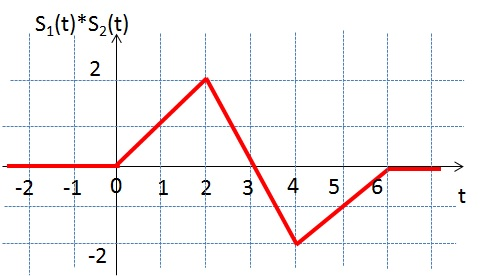
\includegraphics[scale=0.6]{images/TD7_exo6_2.jpg} 
	\end{figure}
	
	
	
	
	\vspace{1\baselineskip}
	
	\subsubsection{Exercice 7 - Échantillonnage}
	
	On considère le circuit de principe ci-dessous, formé d'un interrupteur idéal et appelé échantillonneur. x(t) est le signal d'entrée, h(t) le signal de commande d'ouverture/fermeture de l'interrupteur, et y(t) le signal de sortie. L'interrupteur est ouvert lorsque la commande est nulle. Il se ferme lorsque la commande h(t) = 1.
	Dans cet exercice, on considère que la commande est formée par un peigne de Dirac de période T. Dans un premier temps, le signal d'entrée est une fonction sinus cardinal, tel que $x(t)=A\cdot \frac{sin(\pi \frac{t}{\tau})}{\pi \frac{t}{\tau}}$.
	
	\begin{figure}[h!]
		\centering
		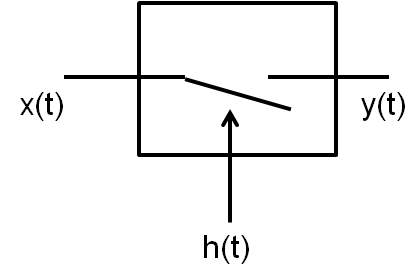
\includegraphics[scale=0.6]{images/Echantillonneur.png} 
	\end{figure}
	
	
	1. Donnez la relation entre les signaux de sortie, d'entrée et de commande.\\
	
	2. Tracez l'allure du signal de sortie. Le nom d'échantillonneur donné au circuit est-il justifié ? Sa présence est-il nécessaire dans un circuit de traitement du signal ?\\
	
	3. Donnez les transformées de Fourier des signaux x(t) et h(t) ? Esquissez leur spectre (en amplitude).\\
	
	4. Déterminez la transformée de Fourier du signal y(t). Esquissez son spectre dans le cas où T << $\tau$, puis dans le cas où T > $\tau$.\\
	
	5. Est-il possible de retrouver le signal x(t) à partir de l'acquisition du signal y(t). Comment et sous quelles conditions ?\\
	
	6. Pourquoi est-il nécessaire de limiter la bande passante des signaux à échantillonner ?
	
	\vspace{1\baselineskip}
	
	\textbf{\underline{Correction exercice 7}}\\
	
	1. On a : $y(t)=h(t)\cdot x(t)$. Comme $h(t)=\sum_{k=-\infty}^{+\infty}\delta(t-kT)$, on a : $y(t)=\sum_{k=-\infty}^{+\infty}x(t-kT)$.	\\
	
	2. L'action de l'échantillonneur provoque un échantillonnage périodique, c'est-à-dire l'acquisition périodique pendant un temps infiniment court de la valeur prise par x(t) à l'instant de l'échantillonnage.
	
	Dans un circuit de traitement du signal, il est nécessaire discrétiser le signal à traiter dans le temps. En effet, pendant le temps du traitement, il est nécessaire de conserver une valeur constante du signal.\\
	
	3. $X(f) = A\tau \Pi_{\frac{1}{\tau}}(f)$. C'est donc un signal dont le spectre est limité sur la bande $[-\frac{1}{2\tau};+\frac{1}{2\tau}]$.
		
	Le signal de commande est un peigne de Dirac, donc un signal périodique, de période T. Le spectre est donc un spectre de raies, dont l'amplitude est donnée par : 
	
	\begin{equation*}
	H_{n}=\frac{1}{T}\int_{-\frac{T}{2}}^{\frac{T}{2}}[\sum_{k=-\infty}^{+\infty}\delta(t-kT)]e^{-j\frac{2\pi n t}{T}}dt
	\end{equation*}
	\begin{equation*}
	H_{n}=\frac{1}{T}\sum_{k=-\infty}^{+\infty}[\int_{-\frac{T}{2}}^{\frac{T}{2}}\delta(t-kT)e^{-j\frac{2\pi n t}{T}}dt]
	\end{equation*}	
	\begin{equation*}
	H_{n}=\frac{1}{T}\int_{-\frac{T}{2}}^{\frac{T}{2}}\delta(t)e^{-j\frac{2\pi n t}{T}}dt
	\end{equation*}
	\begin{equation*}
	H_{n}=\frac{1}{T}
	\end{equation*}
	
	On peut donc écrire : $H(f)=\frac{1}{T}\sum_{k=-\infty}^{+\infty}\delta(f-\frac{k}{T})$. Le spectre d'un peigne de Dirac est un peigne de Dirac.\\
	
	4. $Y(f)=\mathcal{F}[h(t)\cdot x(t)]=H(f)*X(f)=\frac{1}{T}\sum_{k=-\infty}^{+\infty}X(f-\frac{k}{T})$. L'échantillonnage produit une périodisation de X(f) dans le domaine spectral. Son spectre est répété tous les $k\frac{1}{T}$.
	
	\begin{figure}[h!]
		\centering
		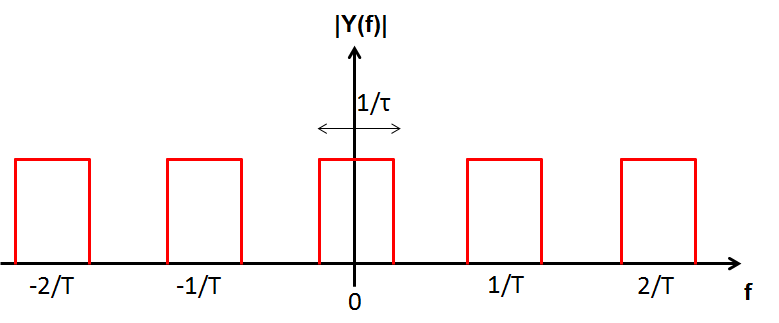
\includegraphics[scale=0.5]{images/TD_7_Exo_7.png} 
	\end{figure}

	5. Sans transformation du signal y(t), il n'est pas possible de revenir au signal x(t), ou au moins à une version s'en rapprochant. Au niveau spectral, si on conserve la partie centrée sur 0 à l'aide d'un filtrage passe-bas, si ce filtre est suffisamment sélectif, on peut retrouver le spectre du signal x(t).
	
	Cependant, cela ne fonctionne que si les différentes répétitions du spectre de X(f) formant Y(f) ne se chevauchent pas (phénomène de recouvrement de spectre). Si on note $F_{max}$ la fréquence maximale d'occupation du spectre X(f) et $F_{e}=\frac{1}{T}$ la fréquence d'échantillonnage, il n'y a pas de recouvrement de spectre si $F_{e} > 2F_{max}$. Il s'agit du théorème de Shannon-Nyquist sur l'échantillonnage.
	
	6. Nous avons fait le raisonnement sur un signal dont le spectre est naturellement limité. On connait parfaitement la fréquence $F_{max}$, donc on peut facilement déterminer la fréquence d'échantillonnage minimale pour respecter le théorème de Shannon-Nyquist. Dans un cas pratique, on connait mal la limite fréquentielle du signal et on risque de créer un problème de recouvrement de spectre. Il est donc recommandé de filtrer le signal pour garantir que le spectre du signal que l'on va échantillonner soit borné. 
	
	
	
	
	\newpage
	
		
	
	\chapter{Energie, puissance et corrélation}
	
	
	\subsubsection{Exercice 1}
	
	Calculez la puissance moyenne et l'énergie totale des signaux suivants :\\
	
	a. $\frac{1}{2}+sin(4\pi t)~,~~t \in \mathbb{R}$\\
	
	b. $cos(\pi t)~,~~t \in [0;3]$\\
	
	c. $e^{-t}u(t)~,~~t \in \mathbb{R}$\\
	
	d. Une impulsion rectangulaire, d'amplitude pic-à-pic de 2 V, centrée en -1 V, d'une durée de 0.1 s et de période égale à 1 s.\\
	
	\textbf{\underline{Correction exercice 1}}\\
	
	a. Signal à puissance moyenne finie, mais énergie infinie.  $\overline{P}=\frac{1}{0.5}\int_{0}^{0.5}(0.5+sin(4\pi t))^{2}dt=\frac{1}{4}+\frac{1}{2}=\frac{3}{4}$\\
	
	b. Signal à énergie totale finie, mais puissance nulle. $E_{tot}=\int_{0}^{3}(cos(\pi t))^{2}dt=\frac{3}{2}$\\
	
	c. Signal à énergie finie mais puissance moyenne nulle. $E_{tot}=\\int_{0}^{+\infty}(e^{-t})^{2}dt=1$\\ 
	
	d. Signal à énergie infinie (périodique) et puissance moyenne finie. $\overline{P}=4x0.1=0.4 W$\\
	
	
	\subsubsection{Exercice 2 - Distorsion harmonique}
	
	On dispose du relevé d'un spectre d'amplitude de raies en sortie d'un système (figure ci-dessous à gauche). Le signal est à support temporel non borné.
	
	\begin{figure}[h!]
		\centering
		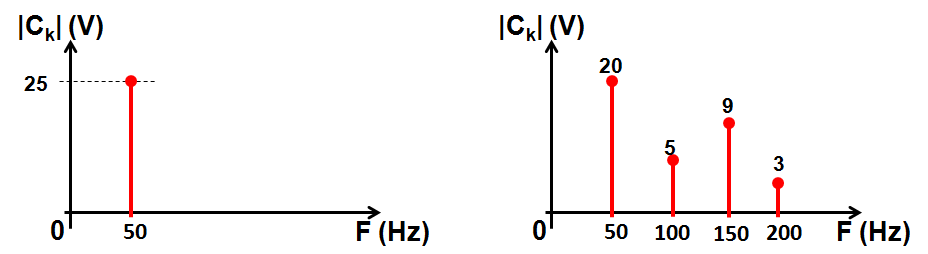
\includegraphics[scale=0.5]{images/Exo_8_2.png} 
	\end{figure}
	
	1. Quelle est la nature du signal ? Précisez ses caractéristiques.\\
	
	2. Quelle est la puissance moyenne du signal ?\\
	
	3. Ce signal traverse un système. On relève le spectre en amplitude en sortie de ce système (figure ci-dessous à droite). Le système est-il linéaire ?\\
	
	4. Calculez la puissance moyenne du signal en sortie du système.\\
	
	5. On définit le taux de distorsion harmonique total (\textit{Total Harmonic Distortion} (THD) en anglais) du signal par rapport au fondamental à l'aide de l'équation suivante :
	\begin{equation*}
	THD_{F}=\frac{\sqrt{\sum_{i=2}^{+\infty}A_{i}^{2}}}{A_{1}}
	\end{equation*}
	
	 avec  $A_{i}$ l'amplitude de l'harmonique de rang i. Calculez ce taux sur les signaux d'entrée et de sortie du système.
	
	\vspace{1\baselineskip}
	
	\textbf{\underline{Correction exercice 2}}\\
	
	1. Puisqu'on observe un spectre de raies, le signal doit être périodique. Puisqu'on ne voit qu'une seule raie à 50 Hz, il s'agit d'un signal (co)sinusoïdal de fréquence 50 Hz. Comme il n'y a pas de raies visibles en f=0, le signal est centré sur 0.\\
	
	2. On utilise l'égalité de Parseval :
	\begin{equation*}
	P_{n}=\frac{1}{T_{0}}\int_{T_{0}}|F(n)|^{2}dt=\|F(1)|^{2}=25^2 = 625 W
	\end{equation*}
	
	3. L'excitation du système par le signal a créé de nouvelles composantes harmoniques. Le système est donc non linéaire.
	
	4. Egalité de Parseval : $P_{n}=\frac{1}{T_{0}}\int_{T_{0}}|F(n)|^{2}dt=\|F(1)|^{2}=20^2+5^2+9^2+3^2 = 515 W$\\
	
	5. Le taux de distorsion harmonique est nul sur le signal d'entrée. Il s'agit d'un signal harmonique pur. En sortie, le taux de distorsion, qui caractérise la non linéarité du système via l'enrichissement du spectre en nouvelles composantes harmoniques, est égale à :
	\begin{equation*}
	THD_{F}=\frac{\sqrt{\sum_{i=2}^{4}A_{i}^{2}}}{A_{1}}=\frac{\sqrt{5^2+9^2+3^2}}{20}=0.53=53 pourcents
	\end{equation*}
	
	
	
	\subsubsection{Exercice 3}
	
	1. Soit le signal porte $x(t)=A\cdot \Pi_{\frac{b}{2}(t)}$, $b\in \mathbb{R^{*}}$.
	
		a. Calculez l'énergie totale et la puissance moyenne du signal.
		
		b. Calculez la fonction d'autocorrélation du signal.
		
		c. Calculez la densité spectrale de puissance ou d'énergie
		
		\vspace{0.5\baselineskip}
	
	2. La fonction x(t) est répétée avec une période T pour former le signal f(t). On prendra $b<\frac{T}{2}$.
	
		a. Calculez l'énergie totale et la puissance moyenne du signal.
		
		b. Calculez la fonction d'autocorrélation du signal.
		
		c. Calculez la densité spectrale de puissance ou d'énergie
	
	\vspace{1\baselineskip}
	
	\textbf{\underline{Correction exercice 3}}\\
	
	1. a. Le signal est à énergie finie : $E_{tot} = 2A^{2}b$. Sa puissance moyenne est nulle.
	
	b. Calcul de la fonction d'autocorrélation :
	\begin{equation*}
	R_{XX}(\tau)=\int_{-\infty}^{+\infty}x(t)x(t-\tau)dt
	\end{equation*}
	\begin{itemize}
		\item si $\tau < -2b$ ou $\tau > 2b$, alors $R_{XX}(\tau)=0$.
		\item si $-2b \leq \tau < 0$, alors $R_{XX}(\tau)=\int_{-b}^{\tau +b}A^{2}dt=A^{2}(\tau+2b)$.
		\item si $0 \leq \tau < 2b$, alors $R_{XX}(\tau)=\int_{\tau-b}^{ b}A^{2}dt=A^{2}(2b-\tau)$. 
	\end{itemize}
	On vérifie que la valeur de l'autocorrélation est l'origine est bien égale à l'énergie totale du signal.

	\begin{figure}[h!]
		\centering
		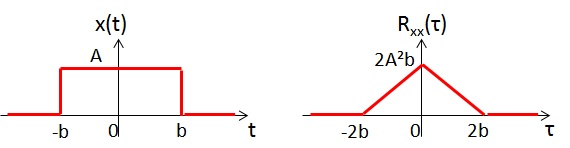
\includegraphics[scale=0.6]{images/Exo_8_1_1.jpg} 
	\end{figure}

	c. Calcul de la densité spectrale d'énergie :
	\begin{equation*}
	S_{X}(f)=\mathcal{F}[R_{XX}(\tau)]=b\cdot sinc(2bf)^{2}\cdot 2A^{2}b=2A^{2}b^{2}sinc(2bf)^{2}	
	\end{equation*}

	\vspace{0.5\baselineskip}
	
	2.a. L'énergie du signal est infinie car il est périodique. Sa puissance moyenne est égale à $\overline{P}=\frac{1}{T}\int_{-\frac{T}{2}}^{\frac{T}{2}}f(t)dt=\frac{2A^{2}b}{T}$. 

	b. La fonction d'autocorrélation est périodique, de période T. Pour chaque période, on trouve :
	\begin{itemize}
		\item pour $-\frac{T}{2}<\tau<-2b$ et $2b<\tau<\frac{T}{2}$,  $R_{FF}(\tau)=0$.
		\item pour $-2b \leq \tau < 0$, alors $R_{YY}(\tau)=\frac{A^{2}(\tau+2b)}{T}$.
		\item si $0 \leq \tau < 2b$, alors $R_{XX}(\tau)\frac{A^{2}(2b-\tau)}{T}$. 
	\end{itemize}
	On vérifie que la valeur de l'autocorrélation est l'origine est bien égale à la puissance moyenne du signal.
	
	\vspace{0.5\baselineskip}
	
	c. La densité spectrale de puissance est donnée par la transformée de Fourier de la fonction d'autocorrélation. Celle-ci étant périodique (fréquence $f_{0}=\frac{1}{T})$, on trouve :
	\begin{equation*}
	S_{F}(f)=\mathcal{F}[R_{FF}(\tau)]=\frac{2A^{2}b^{2}}{T}\sum_{n=-\infty}^{+\infty}sinc(2bnf_{0})\delta(f(-nf_{0}))
	\end{equation*}
	
	
	\vspace{1\baselineskip}	
	
	\subsubsection{Exercice 4}
	
	Un signal noté $x(t)=cos(2\pi f_{0}t)$ excite un filtre passe-bas d'ordre 1, dont la fréquence de coupure est $f_{0}$. Le signal en sortie du filtre est noté y(t).
	
	\vspace{0.5\baselineskip}	
	
	1. Donnez l'expression de la transformée de Fourier X(f) du signal x(t). Tracez son module et son argument.
	
	\vspace{0.5\baselineskip}
	
	2. Donnez l'expression de la fonction de transfert H(f) du filtre. Tracez son module et son argument dans le diagramme de Bode. Quel est son gain et son déphasage en $f_{0}$ ?
	
	\vspace{0.5\baselineskip}
	
	3. A partir de X(f) et H(f), déterminez la transformée de Fourier Y(f) du signal y(t).
	
	\vspace{0.5\baselineskip}
	
	4. Déterminez l'expression du signal y(t) à partir de Y(f).
	
	\vspace{0.5\baselineskip}
	
	5. Calculez la puissance moyenne du signal d'entrée. En déduire celle du signal de sortie.
	
	\vspace{1\baselineskip}	
	
	\subsubsection{Correction exercice 4}
	
	1. $X(f)=\frac{1}{2}(\delta(f-f_{0})+\delta(f+f_{0}))$
	
	
	2. $H(f)$$\frac{1}{1+j\frac{f}{f_{0}}}$. Par convention, le module et la phase sont tracés uniquement pour les fréquences positives dans le diagramme de Bode. Il est intéressant de les tracer aussi pour les fréquences négatives, pour la suite de l'exercice.
	
	En $f= f_{0}$, on a $|H(f_{0})|=\frac{1}{\sqrt{2}}$ et $Arg(H(f_{0}))=-\frac{\pi}{4}$.
	
	3. \begin{equation*}
	Y(f)=H(f)X(f)=\frac{1}{2}(H(f_{0})\delta(f-f_{0})+H(-f_{0})\delta(f+f_{0}))
	\end{equation*}
	\begin{equation*}
	Y(f)=\frac{1}{2}(\frac{1}{1-j}\delta(f-f_{0})+\frac{1}{1+j}\delta(f+f_{0}))
	\end{equation*}
	\begin{equation*}
	Y(f)=\frac{1}{2\sqrt{2}}(e^{-j\frac{\pi}{4}}\delta(f-f_{0})+e^{j\frac{\pi}{4}}\delta(f+f_{0}))
	\end{equation*}

	
	4. On détermine l'expression de y(t) à partir de la transformée de Fourier inverse de Y(f):
	
	\begin{equation*}
	y(t)=\mathcal{F}^{-1}[Y(f)]=\int_{-\infty}^{+\infty}\frac{1}{2\sqrt{2}}(e^{-j\frac{\pi}{4}}\delta(f-f_{0})+e^{j\frac{\pi}{4}}\delta(f+f_{0}))e^{j2\pi ft}df
	\end{equation*}
	
	En utilisant la propriété d'échantillonnage de l'impulsion de Dirac :
	\begin{equation*}
	y(t)=\frac{1}{2\sqrt{2}}(e^{j(2\pi f_{0}t-\frac{\pi}{4})}+(e^{-j(2\pi f_{0}t-\frac{\pi}{4})})
	\end{equation*}
	\begin{equation*}
	y(t)=\frac{1}{\sqrt{2}}cos(2\pi f_{0}t-\frac{\pi}{4})
	\end{equation*}
	
	Le filtre atténue bien le signal d'un facteur $\frac{1}{\sqrt{2}}$ et introduit un déphasage négatif de $-\frac{\pi}{4}$.
	
	\vspace{0.5\baselineskip}	
	
	5. On peut calculer la puissance moyenne $\overline{P_{X}}$ du signal d'entrée à partir de sa densité spectrale de puissance :
	\begin{equation*}
	S_{X}(f)=|X(f)|^{2}
	\end{equation*}
	\begin{equation*}
	\overline{P_{X}}=\int_{-\infty}^{+\infty}S_{X}(f)df=\int_{-\infty}^{+\infty}\frac{1}{4}|\delta(f-f_{0})+\delta(f+f_{0})|^{2}df
	\end{equation*}
	\begin{equation*}
	\overline{P_{X}}=\int_{-\infty}^{+\infty}\frac{1}{4}(\delta(f-f_{0})+\delta(f+f_{0}))df=\frac{1}{2}
	\end{equation*}
	On peut confirmer ce résultat en intégrant le signal temporel sur une période.
	
	On peut calculer la puissance moyenne du signal de sortie à partir de sa densité spectrale de puissance :
	\begin{equation*}
	S_{Y}(f)=|Y(f)|^{2}=|H(f)|^{2}S_{X}(f)
	\end{equation*}
	\begin{equation*}
	\overline{P_{Y}}=\int_{-\infty}^{+\infty}S_{Y}(f)df=\int_{-\infty}^{+\infty}\frac{1}{4}|H(f)|^{2}|\delta(f-f_{0})+\delta(f+f_{0})|^{2}df
	\end{equation*}
	\begin{equation*}
	\overline{P_{Y}}=\frac{1}{4}\int_{-\infty}^{+\infty}|H(f)|^{2}(\delta(f-f_{0})+\delta(f+f_{0}))df=\frac{1}{4}(|H(f_{0})|^{2}+|H(-f_{0})|^{2})
	\end{equation*}
	Le filtre étant réel, on a $|H(f_{0})|=|H(-f_{0})|$, donc on trouve : 
	\begin{equation*}
	\overline{P_{Y}}=\frac{1}{4}2|H(f_{0})|^{2}=\frac{1}{2}(\frac{1}{\sqrt{2}})^{2}=\frac{1}{4}
	\end{equation*}
	Le filtre atténuant l'amplitude d'entrée d'un facteur $\frac{1}{\sqrt{2}}$, la puissance du signal de sortie est donc divisée par 2.
	
	\vspace{1\baselineskip}	
	
	\subsubsection{Exercice 5 - Détection de discontinuité}
	
	On considère un signal x(t) avec plusieurs discontinuités, par exemple : $x(t)=u(t)-2u(t-4)+u(t-6)$. On se propose de trouver une méthode basée sur un calcul d'intercorrélation pour détecter la position de ces discontinuités. On utilise comme signal de détection la fonction $y(t)=sin(2\pi t)(u(t)-u(t-1))$.\\
	
	1. Esquissez l'allure des signaux x(t) et y(t).\\
	
	2. Déterminez l'expression de l'intercorrélation $R_{xy}(\tau)$ entre les signaux x(t) et y(t).Tracez son évolution temporelle. Les discontinuités sont-elles détectées ? Peut-on détecter leur polarité ?\\
	
	3. On choisit un nouveau signal de détection : $y(t)=sin(2\pi \frac{t}{8})(u(t)-u(t-4))$. Reprendre la question précédente. Comment améliorer la précision de la détection ? \\
	
	4. Le dispositif de détection est-il sensible au bruit ?\\
	
	\vspace{1\baselineskip}	
	
	\subsubsection{Exercice 6 - Radar}
	
	La figure ci-dessous illustre le principe de détection d'une cible par le traitement d'un écho radar, et l'estimation de sa distance.
	
	Le radar transmet un signal connu, noté u(t), qui se propage à une vitesse v. Son autocorrélation $R_{u}(\tau)$ est connu. Si un obstacle intercepte ce signal, il en réfléchit une partie. Celle-ci repart en arrière et atteint le radar un temps $t_{1}$ après son émission. Le radar mesure alors l'écho du signal u(t), noté x(t). Celui-ci est la superposition d'une version atténuée du signal u(t) (on supposera l'atténuation constante et on la notera a) et d'un bruit b(t), lié au bruit de mesure et aux interférences électromagnétiques externes.\\
	
	\begin{figure}[h!]
		\centering
		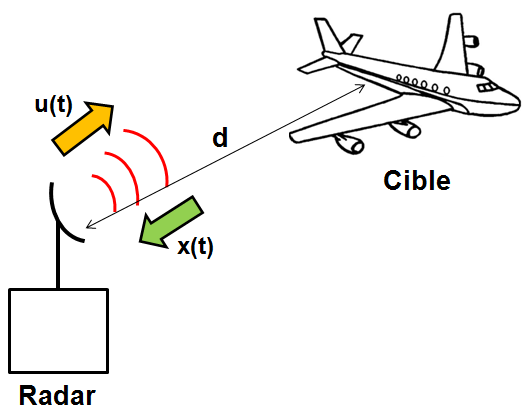
\includegraphics[scale=0.5]{images/TD_8_6.png} 
	\end{figure}
	
	1. Proposez une relation entre les signaux x(t), u(t) et b(t).\\
	
	2. Calculez le produit de convolution : $x(t)*u(-t)$.\\
	
	3. Exprimez l'intercorrélation entre les signaux u(t) et x(t). Exprimez-la en fonction d'autres termes de corrélation.\\
	
	4. Que devient cette expression si le signal de bruit est faiblement corrélé avec le signal u(t) ?\\
	
	5. Proposez une méthode d'estimation de la distance de la cible à partir de la mesure de l'écho du signal radar.\\
	
	6. Quelles propriétés doit vérifier le signal u(t) pour améliorer la précision de la détection ?
	
	
	\vspace{1\baselineskip}	
	
	\textbf{\underline{Correction exercice 6}}\\
	
	1. $x(t)=a\cdot u(t-t_{1})+b(t)$\\
	
	2. $x(t)*u(-t)=(a\cdot u(t-t_{1})+b(t))*u(-t)=a\cdot u(t-t_{1}*u(-t)+b(t)*u(-t)$\\
	On peut remarquer que : $u(t-t_{1})=u(t)*\delta(t-t_{1})$. L'expression du produit de convolution devient :
	\begin{equation*}
	x(t)*u(-t)=a\delta(t-t_{1})*u(t)*u(-t)+b(t)*u(-t)
	\end{equation*}
	
	3. Le produit de convolution précédent n'est rien d'autre que la fonction d'intercorrélation entre x(t) et u(t). On remarque aussi que $u(t)*u(-t)$ correspond à la fonction d'autocorrélation $R_{u}(\tau)$ de u(t), et que $b(t)*u(-t)$ est la fonction d'intercorrélation entre u(t) et b(t), que l'on note $R_{bu}(\tau)$. La relation précédent s'écrit donc :
	\begin{equation*}
	R_{xu}(\tau)=a\delta(\tau-t_{1})*R_{u}(\tau)+R_{bu}(\tau)
	\end{equation*}
	
	Le produit de convolution avec l'impulsion de Dirac conduit à un décalage temporel de $t_{1}$, donc : 
	
	\begin{equation*}
	R_{xu}(\tau)=aR_{u}(\tau-t_{1})+R_{bu}(\tau)
	\end{equation*}
	
	4. Si le bruit est faiblement corrélé avec le signal u(t), son intercorrélation doit être faible. Si elle est suffisamment faible, l'intercorrélation entre u(t) et x(t) doit pouvoir se simplifier :
	\begin{equation*}
	R_{xu}(\tau) \simeq aR_{u}(\tau-t_{1})
	\end{equation*}
	
	5. L'intercorrélation entre x(t) et u(t) est une version atténuée de l'autocorrélation de u(t) et décalée d'un temps $t_{1}$. Or, la fonction d'autocorrélation $R_{u}(\tau)$ présente un maximum en $\tau=0$, donc la fonction $R_{u}(\tau-t_{1})$ présente un maximum en $\tau=t_{1}$. Il en résulte que la fonction $R_{xu}(\tau)$ présente aussi un maximum en $\tau=t_{1}$.
	
	En calculant l'intercorrélation entre x(t) et u(t), on doit trouver un maximum apparaissant en $\tau=t_{1}$, soit le temps d'aller-retour du signal. La distance entre le radar et la cible est donc de : 
	\begin{equation*}
	d=\frac{1}{2}v\cdot t_{1}
	\end{equation*}
	
	L'avantage de cette méthode par rapport à une analyse directe du signal x(t) est que la contribution du bruit est atténuée, et qu'un pic indique l'instant de réception de l'écho.\\
	
	6. Cette technique gagne en précision si :
	\begin{itemize}
		\item le signal u(t) et le bruit b(t) sont faiblement corrélés.
		\item le signal u(t) a une durée faible, pour réduire la largeur du pic mesuré sur la fonction d'intercorrélation.
		\item le signal a une énergie suffisamment forte pour que le pic ressorte du seuil de bruit de la fonction d'intercorrélation 
	\end{itemize}
	
\end{document}